\documentclass[utf8, seminar, numeric, lmodern]{feri}

\renewcommand{\familydefault}{\sfdefault}	% sans-serif main
%\usepackage{inconsolata}					% sans-serif monospace
\usepackage[scaled]{beramono}				% sans-serif monospace

\raggedright						% bez desnog poravnavanja
\usepackage{caption}
\captionsetup{%
	justification=raggedright,
}
\setlength{\parindent}{1em}			% uvlačenje ulomaka
\usepackage{indentfirst}			% uvlačenje prvog ulomka
\setlength{\parskip}{0.5em}			% razmak između ulomaka

\usepackage[T1]{fontenc}  % accented characters, copy from pdf, ...

\usepackage{listings}					% listings
\renewcommand{\lstlistingname}{Ispis}
%\usepackage{floatrow} 				% centriranje svih slika
\usepackage{float}					% figure [H]
\usepackage{graphicx} 				% includegraphics
	\usepackage{caption}			% subfigure
	\usepackage{subcaption}			% subfigure
	\usepackage[export]{adjustbox} 	% http://ctan.org/pkg/adjustbox
	\graphicspath{ {./ilustracije/} }		% mapa sa slikama
	\let\oldincludegraphics\includegraphics
	\renewcommand{\includegraphics}[2][]{\oldincludegraphics[#1,max width=0.9\linewidth]{#2}}
\usepackage{tikz} 					% dijagrami
  \tikzset{>=latex}
  \usepackage{pgfplots}
	  \pgfplotsset{every axis/.append style={
	  		axis x line=middle,    	% put the x axis in the middle
	  		axis y line=middle,    	% put the y axis in the middle
	  		axis line style={->},  	% arrows on the axis
	  		xlabel={$x$},          	% default put x on x-axis
	  		ylabel={$y$},          	% default put y on y-axis
	  		samples=100,
	  		axis equal,
	  	}} % axis style
	\usetikzlibrary{fit}
	
\usetikzlibrary{automata,arrows,positioning,calc}
\usetikzlibrary{arrows,%
	petri,%
	topaths}%
	
\usepackage[croatian]{babel}		% teorem

\usepackage{amsmath}

\usepackage{commath}  % abs, norm, derivacije (\od[2]{f}{x}, \od[2]{f}{x} \dif x = dx)


\usepackage{bm}

%\newtheorem{definition}{Definicija}[section]
%\newtheorem{theorem}{Teorem}[section]
%\newtheorem{corollary}{Korolar}[theorem]

\DeclareMathOperator{\step}{step}
\DeclareMathOperator{\Heaviside}{H}
\DeclareMathOperator{\Ramp}{R}
\DeclareMathOperator{\softplus}{softplus}
\DeclareMathOperator{\softmax}{softmax}
\DeclareMathOperator{\logistic}{\sigma}

\newcommand{\mat}[1]{\bm{#1}}
%\newcommand{\m}[1]{\bm{#1}}
\let\vec\relax
\newcommand{\vec}[1]{\bm{#1}}
%\newcommand{\v}[1]{\bm{#1}}
\newcommand{\tens}[1]{\bm{\mathsf{#1}}} 	% undergraduate algebra version

\newcommand{\transpose}{\mathsf T} 	% undergraduate algebra version

\newcommand{\pderiv}[2]{\frac{\partial #1}{\partial #2}}
\newcommand{\deriv}[2]{\frac{\partial #1}{\partial #2}}  % TODO

\DeclareMathOperator*{\argmin}{arg\,min} % thin space, limits underneath in displays
\DeclareMathOperator*{\argmax}{arg\,max} % thin space, limits underneath in displays

\DeclareMathOperator{\sgn}{sgn}

\usepackage{stmaryrd}  % llbracket \rrbracket, ...


\usepackage[italic]{mathastext}  	% sans-serif math
\usepackage{tabularx}
\usepackage{multirow}

\usepackage[multiple]{footmisc}		% višestruke fusnote

\usepackage{dirtree}

\usepackage[hidelinks]{hyperref}

\usepackage{xcolor}
\hypersetup{
	colorlinks,
	linkcolor={blue!50!green!50!black},
	citecolor={green!40!black},
	urlcolor={blue!75!green!30!black}
}

\usepackage[]{algorithmic}

\usepackage{color}
\definecolor{bluekeywords}{rgb}{0.13,0.13,1}
\definecolor{greencomments}{rgb}{0,0.5,0}
\definecolor{redstrings}{rgb}{0.9,0,0}
\renewcommand*{\UrlFont}{{\small}}

\newcommand{\ilustracija}[1]{\input{ilustracije/#1}}
%\newcommand{\oldnameref}[1]{\nameref{#1}}
%\renewcommand{\nameref}[1]{\emph{\oldnameref{#1}}}  %TODO: ne radi

\begin{document}

% TODO: Navedite broj rada. 


\title{Duboka arhitektura za jednoprolaznu lokalizaciju objekata}

\author{Ivan Grubišić}
\voditelj{Voditelj: Siniša Šegvić}

\maketitle

% Ispis stranice s napomenom o umetanju izvornika rada. Uklonite naredbu \izvornik ako želite izbaciti tu stranicu.
\thispagestyle{empty}
\clearpage
{
	\hypersetup{linkcolor=black}
	\tableofcontents
}


%% Sadržaj seminara

\chapter{Uvod}
Važna skupina problema kojima se bavi računalni vid je razumijevanje slike. Ono najčešeće uključuje klasifikaciju (prepoznavanje) - pridjeljivanje slike odgovarajućem semantičkom razredu (kategoriji ili klasi). Česta poopćenja problema klasifikacije slike su semantička segmentacija i pronalaženje \footnote{U literaturi na engleskom jeziku koriste se izrazi detection i localization. I jedan i drugi često	označavaju različite probleme pronalaženja objekata - ponekad objekti pripadaju jednom razredu, ponekad se traži samo jedan objekt, a ponekad se traži i klasificira veći broj objekata, od čega je ovo zadnje tema ovog seminara.} objekata. Semantička segmentacija je klasificiranje svakog dijela (piksela) slike. Pronalaženje objekata se sastoji od pronalaženja okvira od kojih svaki uokviruje jedan objekt i klasifikaciju svakog od njih. Postoji i pristup koji ujedinjuje navedena dva - semantička segmentacija uz razlikovanje objekata. 

U posljednjih nekoliko godina postiže se značajan napredak u računalnom vidu. On se uglavnom temelji na razvoju dubokih konvolucijskih mreža u kojima glavnu ulogu imaju konvolucijski slojevi. Istovrsni objekti mogu se na slici pojavljivati na različitim položajima na slici. Konvolucijske arhitekture neuronskih mreža iskorištavaju to svojstvo tako da se isti neuron unutar nekog sloja može učiti i koristiti na svim položajima ulazne slike (ili sloja).

U poglavlju \ref{chap:konv-nn} opisani su osnovni pojmovi vezani uz konvolucijske mreže s naglaskom na konvolucijski sloj. To poglavlje je zasnovano na razradi te teme u završnom radu \cite{semseg-ja}. U poglavlju \ref{chap:detekcija} opisan je problem pronalaženja objekata na slici i dan je pregled glavnih pristupa rješavanju tog problema. U poglavlju \ref{chap:ssd} opisan je postupak SSD \cite{ssd}. U poglavlju \ref{chap:rezultati} pokazani su primjeri rezultata sustava SSD i usporedba rezultata s drugim modelima. U poglavlju \ref{chap:zakljucak} je zaključak.

\chapter{Konvolucijske mreže} \label{chap:konv-nn}
% http://cs231n.github.io/convolutional-networks/#conv
% http://andrew.gibiansky.com/blog/machine-learning/convolutional-neural-networks/
Konvolucijske mreže su unaprijedne neuronske mreže koje se sastoje od većeg broja slojeva prilagođenih obradi signala koji u različitim položajima mogu sadržavati slične uzorke. One omogućuje efikasno učenje i obradu i posebno se uspješno primjenjuju u računalnom vidu.

Kod općenite višeslojne unaprijedne neuronske mreže svaki skriveni sloj sastoji se od neurona koji su potpuno povezani s neuronima prethodnog sloja i od kojih svaki ima težine neovisne o težinama drugih neurona. Takva bi mreža za ulaze većih dimenzija poput slika imala prevelik broj parametara, teško bi učila i bila bi sklona prenaučenosti. 

Kod konvolucijskih mreža slojevi su rijetko i lokalno povezani i koriste dijeljenje parametara. Svaki neuron povezan je s malim brojem bliskih neurona prethodnog sloja. Osnovna građevna jedinica konvolucijske mreže je konvolucijski sloj. Njega čini skup naučenih filtara od kojih svaki stvara jednu matricu izlaznog tenzora značajki. Te matrice se nazivaju mapama značajki. Filtri se još nazivaju konvolucijskim jezgrama i općenito su trodimenzionalni. Imaju dvije prostorne dimenzija i jednu koja se općenito proteže kroz sve mape značajki ulaznog tenzora. Pomicanjem filtra po prostornim dimenzijama generira se jedna od izlaznih mapa značajki.

Za klasifikaciju se na kraju mreže obično koristi jedan ili više potpuno povezanih slojeva ili konvolucijski sloj i globalno sažimanje aritmetičkom sredinom. Izlaz takvog konvolucijskog sloja sadrži jednu mapu značajki za svaki razred. Globalno sažimanje aritmetičkom sredinom svaku mapu značajki preslikava u njenu aritmetičku sredinu, čime se dobiva jedna vrijednost za svaki razred. Unutar mreže se nalaze posebni konvolucijski slojevi ili slojevi sažimanja koji služe smanjenju prostornih dimenzija tenzora značajki (među ostalim mogućim ulogama).

Parametri konvolucijskih mreža uče se, slično kao kod klasičnih neuronskih mreža, algoritmom propagacije pogreške unatrag (engl. \emph{backpropagation}) koji se temelji na pravilu derivacije složene funkcije i dinamičkom programiranju.


\section{Konvolucijski slojevi} \label{sec:konv-sloj}

Svojstva konvolucijskih slojeva temelje se na pretpostavci da se istovrsni uzorci mogu pojavljivati na svim položajima u ulazu. To se ostvaruje dijeljenjem parametara između neurona unutar nekog sloja. Djelovanje takvog sloja može se predstaviti konvolucijama dijeljenih težina s ulaznim tenzorom, dodavanjem pragova i primjenom prijenosne funkcije. Na slici~\ref{fig:lok_pov} prikazan je jedan jednostavan konvolucijski sloj.

\begin{figure}[htbp] \centering
	\ilustracija{konv-sloj}
	\caption{Primjer jednostavnog jednodimenzionalnog konvolucijskog sloja s jednom ulaznom i jednom izlaznom mapom značajki. Svaka izlazna vrijednost se računa na temelju vrijednosti oko istog položaja pomnoženih težinama i dodanim pragom. Težine i prag su zajednički svim neuronima. Iste težine su naznačene jednako tamnim strelicama.}
	\label{fig:lok_pov}
\end{figure}

Kod dvodimenzionalnih konvolucijskih slojeva kakvi se koriste u računalnom vidu težine se mogu predstaviti matricama koje se filtrima ili konvolucijskim jezgrama (engl. \emph{kernel}). Jedna izlazna mapa značajki se dobiva konvolucijom pripadajuće konvolucijke jezgre s mapama značajki ulaznog tenzora po prostornim dimenzijama, zbrajanjem i primjenom prijenosne funkcije. Dalje će se $n$-torka dvodimenzionalnih jezgri, gdje je $n$ općenito broj ulaznih mapa značajki, samo zvati jezgrom. Koriste se jezgre malih prostornih dimenzija, često $1\times 1$, $3\times3$ ili $5\times5$.

Konvolucija se provodi pomicanjem jezgre po prostornim dimenzijama (visina i širina) prethodnog sloja i zbrajanjem praga i umnožaka elemenata jezgre s odgovarajućim vrijednostima mapa značajki prethodnog sloja. Na rezultate konvolucije s više različitih jezgri primjenjuje se prijenosna funkcija i dobivaju se konačne izlazne mape značajki. Svaka mapa značajki predstavlja ulaz filtriran na drugačiji način, s prepoznatim drugačijim značajkama. To se može izraziti ovako:
\begin{equation}
\matr{H}_{lp}=\varphi\left(
-\theta_{lp} + \sum_q \matr{w}_{lpq}\ast\matr{H}_{(l-1)q}\right).
\end{equation}
Ovdje $\matr{H}_{lp}$ označava $p$-tu izlaznu mapu značajki sloja $l$, $\matr{H}_{(l-1)q}$ ulazne mape značajki s rednim brojevima $q$, $\theta_{lp}$ odgovarajući prag, a $\matr{w}_{lpq}$ $q$-tu komponentu odgovarajuće jezgre pridruženu $q$-toj mapi značajki sloja $l-1$. $\varphi$ predstavlja prijenosnu funkciju, a $\ast$ označava operator konvolucije koji može biti definiran ovako:
\begin{equation}
(\matr{h}\ast\matr{x})_{mn} = \sum_i \sum_j h_{ij} x_{(m-i)(n-j)},
\end{equation}
gdje su $\matr{h}$ i $\matr{x}$ matrice (s pomaknutim koordinatama) ili funkcije $\mathbb{Z}\times\mathbb{Z}\rightarrow\mathbb{R}$.

Na slici~\ref{fig:konv} prikazan je primjer konvolucije jedne mape značajki i dvodimenzionalne jezgre koja prepoznaje vertikalne rubove. U slučaju da se ulaz sastoji od više komponenata, izlazna matrica jednaka je zbroju rezultata konvolucija svih komponenata s odgovarajućim komponentama konvolucijske jezgre.

\begin{figure}[htbp] \centering
	\ilustracija{konv}
	\caption{Primjer jednostavne dvodimenzionalne diskretne konvolucije (jedna jezgra dimenzija $2\times 2\times 1$) kojom se stvara jedna mapa značajki na temelju jedne ulazne mape značajki}
	\label{fig:konv}
\end{figure}

Kao prijenosna funkcija kod konvolucijskih slojeva najčešće se koristi zglobnica (engl. \emph{Rectified linear unit}, \emph{ReLU}) definirana ovako:
\begin{equation}
\varphi(x) = \max(0, x).
\end{equation}

Kako bi izlazne mape značajki bile jednake širine i visine kao ulaz, potrebno je nekako nadopuniti ulaz na mjestima na kojima konvolucijska jezgra prelazi njegove rubove. Rubovi ulaza se najčešće nadopunjuju nulama. Ponekad se jezgra umjesto jedan po jedan piksel pomiče po više piksela odjednom, čime se smanjuju dimenzije izlaza. Taj pomak nazivamo izlazni korak (engl. \emph{stride}).


\section{Smanjivanje dimenzija slojeva} \label{sec:smanjivanje-dimenzija}

U konvolucijskim mrežama je važno smanjiti broj parametara i veličine slojeva kako bi se smanjili memorijski zahtjevi modela i ubrzalo izvođenje. To se ostvaruje smanjivanjem dimenzija slojeva i korištenjem manjih konvolucijskih filtara. Za smanjivanje dimenzija slojeva (mapa značajki) donedavno su se uglavnom koristili slojevi sažimanja. Najčešće vrste sažimanja su sažimanje maksimalnom vrijednošću (engl. \emph{max-pooling}) i sažimanje srednjom vrijednošću (engl. \emph{average-pooling}). 

Slojevi sažimanja najčešće ostvaruju sažimanje maksimalnom vrijednošću ili aritmetičkom sredinom. Jednostavan primjer sažimanja maksimalnom vrijednošću kojim se dimenzije ulazne mape značajki smanjuju na pola prikazan je na slici~\ref{fig:max_pool}. Dimenzije tih četverokuta su najčešće $2\times2$, čime se širina i visina ulaza dvostruko smanjuju. Sažimanje se provodi na svakoj mapi značajki nezavisno pa je broj mapa značajki izlaznog tenzora jednak broju mapa značajki ulaznog tenzora.

\begin{figure}[htbp] \centering
	\ilustracija{max_pool}
	\caption{Sažimanje maksimalnom vrijednošću}
	\label{fig:max_pool}
\end{figure}

U novijim uspješnim modelima~\cite{resnet}, a posebno u nenadziranim generativnim modelima~\cite{gan}, često se umjesto navedenih slojeva sažimanja koriste konvolucijski slojevi s izlaznim korakom većim od $1$. Ako je izlazni korak konvolucije $n$, konvolucijski filtri se, umjesto na svakom položaju ulaznih mapa značajki, postavljaju na svaki $n$-ti položaj u pojedinoj prostornoj dimenziji. Time se postiže da se dimenzije izlaznih mape značajki uz izlazni korak $n$ smanjuju na $1/n$ odgovarajućih dimenzija ulaza.



\chapter{Lokalizacija objekata} \label{chap:detekcija}

Jedan od osnovnih problema računalnog vida je klasifikacija slika, tj. prepoznavanje vrste (razreda) objekta koji se nalazi na slici. Skup podataka za učenje klasifikacije slika sastoji se od slika i oznaka razreda od kojih je svaka pridružena jednoj slici. Izlaz sustava za klasifikaciju je obično vektor koji predstavlja razdiobu vjerojatnosti pripadanja primjera svakom od razmatranih razreda, tj pouzdanosti (engl. \emph{confidence}) klasifikacije.

Kod pronalaženja objekata zadatak je prepoznati svaki objekt na slici koji pripada poznatom razredu i pridružiti mu oznaku njegovog razreda i najmanji opisani pravokutnik ili okvir (engl. \emph{minimum bounding box}, \emph{oriented bounding box}) unutar kojeg se nalazi. Skup podataka za učenje postupaka za pronalaženje objekata se sastoji od slika i svakoj od njih pridruženog skupa okvira s odgovarajućim oznakama razreda\footnote{Postoji i jednostavniji problem pronalaženja samo jedne vrste objekata pa u tom slučaju oznake razreda ne bi bile potrebne.}. Na slici~\ref{fig:det-obj} prikazan je primjer rezultata sustava za pronalaženje objekata na jednoj slici.

\begin{figure}[htbp] \centering
	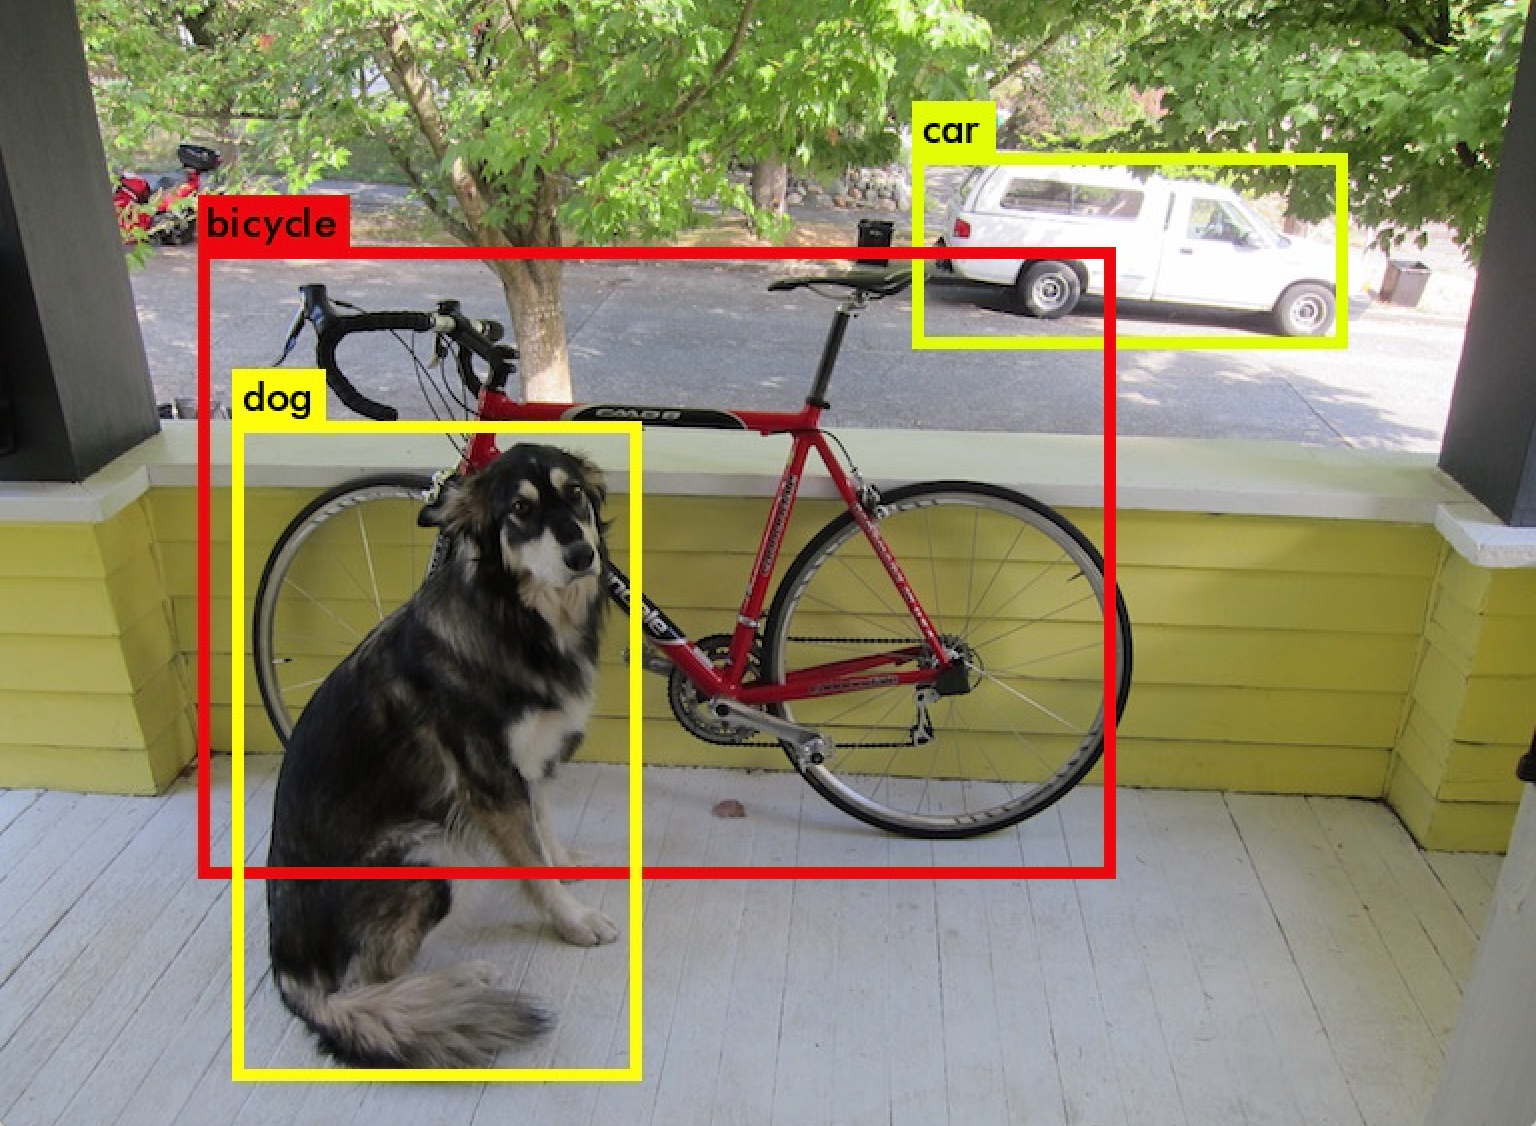
\includegraphics[max width=1\linewidth]{object-detection.png}
	\caption{Primjer slike iz~\cite{yolo2web} s objektima kojima su pridruženi okviri.}
	\label{fig:det-obj}
\end{figure}


\section{Osnovni pristupi}

Uz riješen problem klasifikacije, najjednostavniji pristup pronalaženju objekata je korištenje pomičnih okana različitih dimenzija i klasificiranje svake na taj način dobivene \emph{podslike}. Na taj način se za neki objekt na slici dobije velik broj okvira unutar kojih se taj objekt prepoznaje s određenom razinom pouzdanosti. Nakon toga potrebno je za svaki objekt pronaći jedan okvir koji ga najbolje opisuje. 

Do otprilike $2012$. godine najuspješniji su bili modeli koji objekte modeliraju dijelovima koji mogu biti različito raspoređeni (engl. \emph{deformable part model}, \emph{DPM})~\cite{objdet2014} i pri tome kao značajke koriste histograme gradijenata (engl. \emph{histogram of gradients}, \emph{HoG}).

%HOG detector: http://www.cs.utoronto.ca/~fidler/slides/CSC420/lecture17.pdf

Malo kasnije su se pokazali uspješnima postupci koji na neki način smanjuju broj okvira koje sustav treba potpuno klasificirati. Na temelju jednostavnijih značajki koje se mogu brže izračunati moguće je odabrati kandidate okvira koji s većom vjerojatnošću opisuju objekte. To se naziva predlaganje okvira (engl. \emph{bounding box proposals}) i time se smanjuje ukupan broj okvira koje treba potpuno klasificirati. Neki primjeri postupaka predlaganja okvira se temelje na segmentaciji slike superpikselima (\emph{Selective search}~\cite{selectiveSearch}), korištenju rubova (\emph{Edge boxes}~\cite{edgeBoxes}) ili konvolucijskoj mreži (\emph{region proposal network}, \emph{RPN}~\cite{fasterrcnn}) koja se može brže izvršavati na grafičkim procesorima. Smanjenje broja okvira koje treba klasificirati omogućuje korištenje jačih modela za učenje značajki i klasifikaciju uz isto ili kraće vrijeme izvođenja. 


\section{Evaluacijske mjere}

\subsection{Jaccardov koeficijent sličnosti}

Kod pronalaženja objekata izlaz sustava je skup (klasificiranih) okvira. Mjera koja se koristi kao mjera kvalitete lokalizacije je omjer površine presjeka i unije ($\mathit{IoU}$, engl. \emph{intersection over union}). Omjer presjeka i unije se još naziva Jaccardov koeficijent sličnosti i označava se s $J$. Vrijednost koeficijenta sličnosti je $1$ ako i samo ako su okviri koje uspoređuje jednaki. Neka su $A$ i $B$ dva okvira koje smatramo skupovima piksela. Onda je koeficijent sličnosti definiran ovako:
\begin{equation}
J(A,B) = \frac{|A\cap B|}{|A\cup B|} = \frac{|A\cap B|}{|A|+|B|-|A\cap B|}.
\end{equation}

\subsection{Preciznost, odziv i srednja prosječna preciznost}

Preciznost ($P$, engl. \emph{precision}) se koristi kao mjera relevantnosti rezultata i jednaka je udjelu relevantnih rezultata u svim rezultatima, a odziv ($R$, engl. \emph{recall}) je udio relevantnih rezultata u svim relevantnim objektima. 

Ako $\mathit{tp}$ (engl. \emph{true positives}) predstavlja broj prepoznatih relevantnih objekata, $\mathit{fp}$ (engl. \emph{false positives}) broj nerelevantnih objekata klasificiranih pod relevantne, a $\mathit{fn}$  (engl. \emph{false negatives}) broj neprepoznatih relevantnih objekata, onda se preciznost i odziv definiraju ovako:
\begin{align}
P &= \frac{\mathit{tp}}{\mathit{tp} + \mathit{fp}}, \\
R &= \frac{\mathit{tp}}{\mathit{tp} + \mathit{fn}}.
\end{align}

Neka je $H$ skup okvira rezultata, a $T$ skup ciljnih okvira. Bez smanjenja općenitosti, neka svi okviri imaju istu oznaku razreda. Neka je $h \in H$ promatrani okvir rezultat. Prema \cite{pascalVOC-devkit}, on se smatra ispravnim (\emph{true positive}) ako postoji $t\in T$ tako da vrijedi $J(t,h) > 0.5$ i $\forall h'\in H \, J(t, h) \geq J(t, h')$. Inače se smatra neispravnim (\emph{false negative}).

Uz položaje i dimenzije okvira, sustav za pronalaženje objekata obično daje i mjeru pouzdanosti klasifikacije okvira. Krenuvši redom od okvira za koji je sustav najsigurniji, uzimanjem u obzir sve više okvira spuštanjem praga pouzdanosti klasifikacije smanjuje se preciznost, a povećava odziv. To se može grafički prikazati krivuljom preciznosti i odziva (slika~\ref{fig:pr-krivulja}).

\begin{figure}[htbp] \centering
	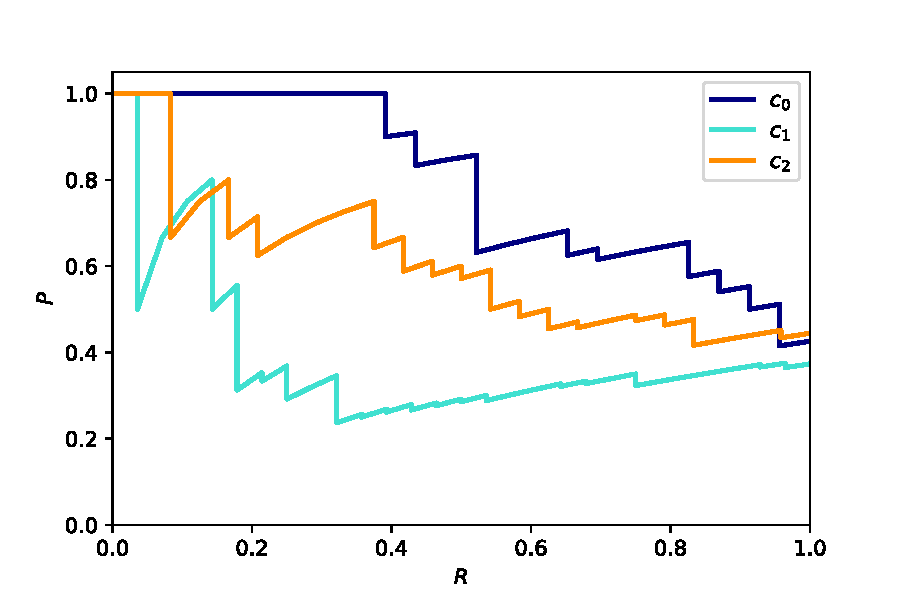
\includegraphics[max width=1\linewidth]{pr-curve.pdf}
	\caption{Primjer krivulja preciznosti i odziva za $3$ razreda. Slika je preuzeta iz~\cite{prec-rec} i prilagođena.}
	\label{fig:pr-krivulja}
\end{figure}

Kao evaluacijska mjera za pronalaženja objekata s jednim razredom se najčešće koristi prosječna preciznost (engl. \emph{average precision}), a u slučaju više razreda srednja prosječna preciznost (engl. \emph{mean average precision}). Preciznije, češće se koristi preciznost interpolirana na monotono padajuću krivulju s obzorom na odziv, što je malo dalje opisano.

Prosječna preciznost je često definirana kao površina ispod krivulje preciznosti i odziva:
\begin{equation} \label{eq:AP}
\mathit{AP} = \int_{0}^{1} P(r) \dif r,
\end{equation}
gdje $r$ predstavlja odzive. Postoje i drugačije definicije~\cite{wiki-ir}.

Srednja prosječna preciznost je, uz skup razreda $C$, definirana ovako:
\begin{equation} \label{eq:mAP}
\mathit{mAP} = \frac{1}{\abs C}\sum_{c \in C} \mathit{AP}_c .
\end{equation}

Češće se ista oznaka $\mathit{mAP}$ koristi za srednju prosječnu interpoliranu preciznost, tj. umjesto preciznosti se koristi preciznost interpolirana na monotono padajuću krivulju (s obzirom na odziv). Neka $P_\mathrm{i}$ označava interpoliranu preciznost, a $r$ odzive. Interpolirana preciznost je definirana ovako:
\begin{equation} \label{eq:Pi}
P_\mathrm{i}(r) := \max\{P(r') \mid r' \geq r \}.
\end{equation}
Na slici~\ref{fig:pr-interp} je prikazana krivulja interpolirane preciznosti u ovisnosti o odzivu.

\begin{figure}[htbp] \centering
	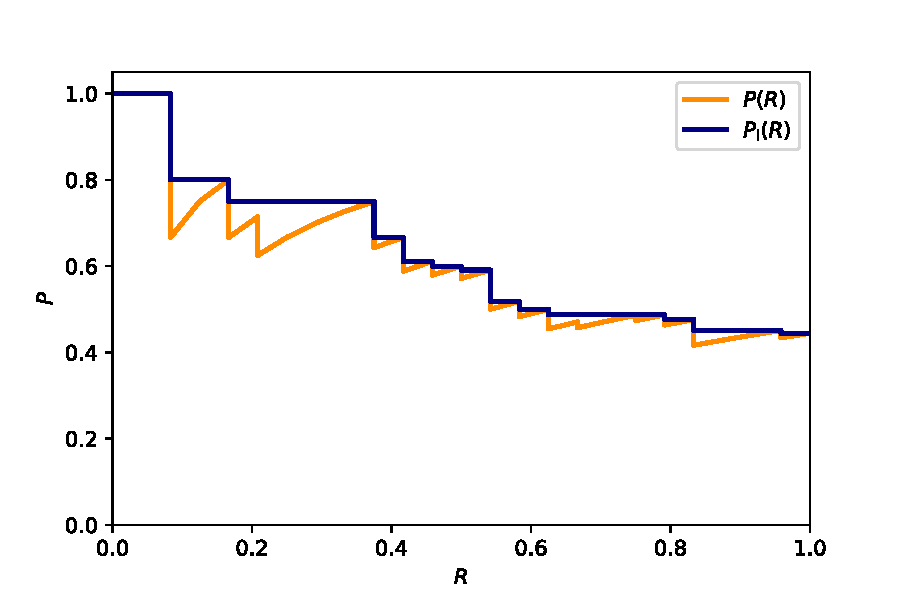
\includegraphics[max width=1\linewidth]{pr-interp.pdf}
	\caption{Primjer krivulje preciznosti u ovisnosti o odzivu (narančasto) i odgovarajuće krivulje interpolirane preciznosti u ovisnosti o odzivu (plavo).}
	\label{fig:pr-interp}
\end{figure}

Dalje u ovom seminaru će se koristiti oznaka $\mathit{mAP}$ za srednju prosječnu interpoliranu preciznost.



\chapter{SSD: Single Shot MultiBox Detector} \label{chap:ssd}

SSD (\emph{Single Shot Multibox Detector})~\cite{ssd} je model za pronalaženje objekata (koji pripadaju većem broju razreda) koji se temelji na dubokoj konvolucijskoj mreži koja u jednoj propagaciji unaprijed generira sve predikcije okvira od kojih se oni najbolji ostavljaju (engl. \emph{single-shot detection}). 

Glavna značajka SSD-a je da umjesto korištenja posebne komponente za generiranje prijedloga okvira koristi ravnomjerno raspoređene okvire (slika~\ref{fig:ssd-default-boxes}) koji će se dalje nazivati razmatranim okvirima i na svima od njih u jednom prolazu provodi klasifikaciju i regresiju položaja i omjera stranica. Za svaki okvir se procjenjuje pouzdanost klasifikacije u moguće razrede i prilagodbe dimenzija i položaja. Još jedna bitna značajka mreže je da dijelovi za prepoznavanje objekata izravno koriste izlazne tenzore značajki konvolucijskih slojeva različitih veličina na različitim dubinama konvolucijske mreže. Time se omogućuje bolje prepoznavanje objekata različitih veličina. Za dodatno poboljšavanje regresije omjera stranica, na istim položajima se koriste razmatrani okviri različitih omjera stranica.

\begin{figure}[htbp] \centering
	\begin{subfigure}[b]{0.32\textwidth} \centering
		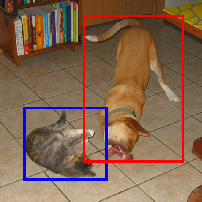
\includegraphics[width=\textwidth]{ssd-truth.pdf}
		\caption{Slika sa željenim okvirima}
	\end{subfigure}
    \begin{subfigure}[b]{0.32\textwidth} \centering
		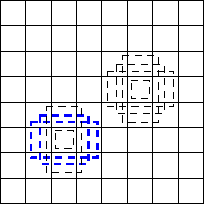
\includegraphics[width=\textwidth]{ssd-8x8fm.pdf}
		\caption{Mapa značajki dimenzija $8\times8$}
	\end{subfigure}
	\begin{subfigure}[b]{0.32\textwidth} \centering
		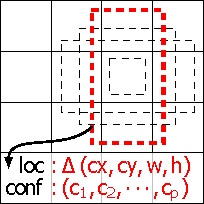
\includegraphics[width=\textwidth]{ssd-4x4fm.pdf}
		\caption{Mapa značajki dimenzija $4\times4$}
	\end{subfigure}
	%TODO: napraviti novu sliku
	\caption{Slike ilustriraju glavne značajke modela SSD. Svakom pikselu nekih slojeva značajki pridruženo je nekoliko razmatranih okvira različitih omjera stranica. Crtkani okviri na prikazanim mapama značajki po položaju, veličini i omjeru stranica najbolje odgovaraju ciljnim okvirima na slici i zato su najpogodniji za učenje parametara na tom primjeru. Slike su preuzete iz \cite{ssd}.}
	\label{fig:ssd-default-boxes}
\end{figure}

Za ulazne slike dimenzija $300\times300$ na skupu podataka VOC2007-test SSD ostvaruje $\mathit{mAP}=0.743$ i brzinu (broj obrađenih slika u sekundi) $59 s^{-1}$ uz paralelizirano obrađivanje 8 slika i $46 s^{-1}$ uz pojedinačno obrađivanje slika na grafičkoj kartici \emph{Nvidia Titan X}, što je poboljšanje za malo više od $0.01$ u $\mathit{mAP}$ i više nego šesterostruko ubrzanje u odnosu na tada\footnote{Rad je objavljen $2016$. godine.} najbolji model Faster R-CNN~\cite{fasterrcnn}.
U međuvremenu su se pojavili još neki modeli koji su dostigli ili prestigli performanse SSD-a~\cite{pvanet, yolov2}. 


\section{Model} \label{sec:ssd-model}

\paragraph{Konvolucijska arhitektura za izlučivanje značajki.}
Model se temelji na prednjem dijelu neke dobre unaprijedne konvolucijske mreže za klasifikaciju. Koriste se svi slojevi te mreže osim onih zadnjih koji služe konačnoj klasifikaciji. U radu je za to korištena mreža VGG-16~\cite{vgg} do sloja \texttt{conv\_5\_3} (bez posljednja dva potpuno povezana sloja za klasifikaciju). Takvoj mreži je dodano još $10$ slojeva od kojih neki koriste izlazni korak $2$ za konvoluciju i prema kraju se (u slučaju modela SSD-300) smanjuju od dimenzija $19\times 19$ do dimenzija $1\times 1$. Ti dodatni slojevi služe prepoznavanju značajki više razine i omogućuju bolje prepoznavanje objekata različitih dimenzija. 

Za lokalizaciju objekata se izravno koriste tenzori značajki $6$ slojeva. Najveći od njih, koji je dimenzija $38\times 38$, je sloj \texttt{conv4\_3} iz mreže VGG-16. Jedan piksel neke njegove mape značajki po relativnoj veličini odgovara otprilike $8\times8$ piksela ulazne slike koja je dimenzija $300\times 300$. Zadnji sloj značajki \texttt{conv11\_2} je dimenzija $1\times 1$ i svaka njegova mapa značajki (od njih 256) sastoji se od samo jedne realne vrijednosti. On se koristi za prepoznavanje objekata koji prekrivaju cijelu sliku. Arhitektura mreže je detaljnije opisana na slici~\ref{fig:ssd-arh}. Kao prijenosna funkcija se za sve konvolucijske slojeve koristi zglobnica ($\mathrm{ReLU}$).

\begin{figure}[htbp] \centering
	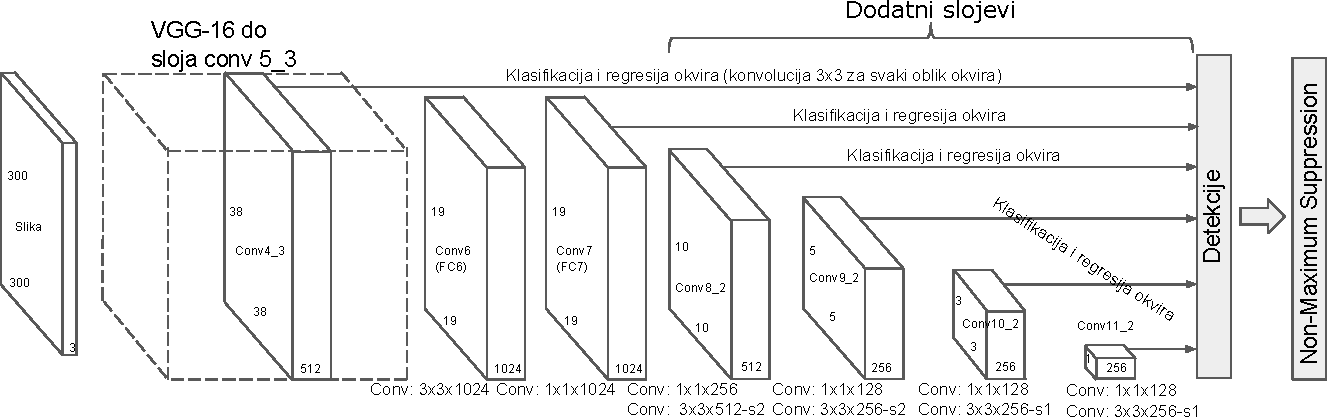
\includegraphics[max width=1\linewidth]{ssd-dijagram.pdf}
	%TODO: napraviti novu sliku
	\caption{Ilustracija sustava SSD s prikazanim mapama značajki koje se koriste za pronalaženje objekata. Slika je preuzeta iz \cite{ssd} i malo izmijenjena.}
	\label{fig:ssd-arh}
\end{figure}

\paragraph{Slojevi za pronalaženje objekata.}
Tenzor značajki sloja \texttt{conv4\_3} (dimenzija $38\times 38\times 512$) i tenzore značajki $5$ od $10$ dodatnih slojeva (dimenzija od $19\times 19\times 1024$ do $1\times 1\times 256$) koriste dijelovi mreže za lokalizaciju, tj klasifikaciju i regresiju razmatranih okvira. Svakom položaju u mapama značajki svakog od tih slojeva pridružen je jedan skup razmatranih okvira različitih dimenzija.
Pomicanjem konvolucijskih jezgri, od kojih svaka predstavlja za jedan oblik okvira, preko tenzora značajki provodi se klasifikacija i regresija razmatranih okvira. Te jezgre su dimenzija $3\times 3\times p$, gdje je $p$ broj mapa značajki ulaznog tenzora. Računaju se pouzdanosti klasifikacije u $\left|C\right|$ razreda i prilagodbe okvira (pomak središta i prilagodba dimenzija\footnote{Vrijednosti prilagodbi okvira nisu apsolutne (u pikselima) nego su relativne s obzirom na razmatrani okvir. Pomak u vertikalnom/horizontalnom smjeru je skaliran inverzom visine/širine razmatranog okvira, a prilagodba visine/širine je prirodni logaritam visine/širine podijelene visonom/širinom razmatranog okvira. To je formalnije opisano u ulomku \nameref{par:ssd-ucenje-gubitak} u potpoglavlju~\ref{sec:ssd-ucenje}.}) kako bi se okviri prilagodili obliku objekta.
Neka je $R$ skup brojeva koji predstavljaju omjere stranica. Iz nekog tenzora značajki na svakom se položaju primjenom $|R|$ konvolucijskih jezgri za klasifikaciju i regresiju okvira dobiva $(|C|+4)\left|R\right|$ vrijednosti koje definiraju pouzdanosti klasifikacije, položaj i dimenzije okvira rezultata.

\paragraph{Veličine i omjeri stranica razmatranih okvira.} \label{par:ssd-model-okviri}
Na slici~\ref{fig:ssd-default-boxes} prikazana su dva primjera slojeva značajki različitih dimenzija i okviri pridruženi nekim njihovim pikselima. Neka se koristi $m$ tenzora značajki za traženje objekata. Faktor skaliranja za okvire $k$-tog sloja značajki, uz $k\in \{1..m\}$, određuje se ovako:
\begin{equation}
\sigma_k = \sigma_\mathrm{min} + \frac{k-1}{m-1}(\sigma_\mathrm{max}-\sigma_\mathrm{min}).
\end{equation}
Pri tome $\sigma_\mathrm{min} = 0.2$ i $\sigma_\mathrm{max}=0.9$. Uz omjere stranica $r\in R=\left\{1,2,3,\frac{1}{2},\frac{1}{3}\right\}$, širine $w_{kr}$ i visine $h_{kr}$ razmatranih okvira $k$-tog sloja značajki nad kojim se primjenjuje klasifikacija i regresija okvira se računaju ovako:
\begin{align}
w_{kr} &= \sigma_k r^{\frac{1}{2}}, \\
h_{kr} &= \sigma_k r^{-\frac{1}{2}}.
\end{align}
Također se još koriste okviri omjera $1$ s faktorom skaliranja $\sigma_k'=\sqrt{\sigma_k \sigma_{k+1}}$. Tako se dobiva $|R|+1=6$ razmatranih okvira za svaki položaj u nekom od odabranih tenzora značajki. 

U konačnom modelu koji je testiran kod nekih slojeva postoje odstupanja od navedenih pravila omjera stranica i faktora skaliranja.

\paragraph{Odbacivanje okvira.}
Za ulaznu sliku dimenzija $300\times 300$ dobije se $8732$ okvira. Većinu njih treba odbaciti i ostaviti samo jedan okvir za svaki objekt pronađen na slici. Za to se koristi algoritam \emph{non-maximim suppression} (\emph{NMS}). Njime se za svaki razred nezavisno pronalaze okviri za koje je Jaccardov koeficijent sličnosti veći od određenog praga i, uzimajući u obzir pozdanosti klasifikacije, pohlepnim algoritmom se uklanja višak okvira. Točna implementacija je dostupna ovdje: \url{https://github.com/intel/caffe/blob/master/src/caffe/util/bbox_util.cpp}.

\section{Učenje} \label{sec:ssd-ucenje}

SSD se uči tako da se za svaku sliku s ciljnim okvirima prvo iz skupa za učenje među razmatranim okvirima odaberu oni koji su najprikladniji za učenje pozitivnih i negativnih primjera rezultata, a onda se parametri korišteni za dobivanje odabranih okvira prilagođavaju algoritmom koji se temelji na gradijentnom spustu. $S$ će dalje označavati skup razmatranih okvira, a $T$ skup ciljnih okvira trenutne slike. $C$ će označavati skup razreda koji uključuje i razred \emph{ostalo} (ili \emph{pozadina}).

\paragraph{Odabir razmatranih okvira za učenje.} Tijekom učenja na nekoj slici potrebno je odrediti koji od razmatranih okvira su po položajima i dimenzijama najprikladniji za učenje parametara. Prvo se za svaki objekt, tj. ciljni okvir, pronalazi razmatrani okvir koji se s njim najviše preklapa, tj. ima najveći Jaccardov koeficijent sličnosti s njim. Tako se osigurava da je svakom objektu pridružen barem $1$ razmatran okvir. Također se još odabiru i drugi razmatrani okviri koji se s nekim ciljnim okvirom preklapaju s Jacardovim koeficijentom većim od $0.5$. Na taj način se pri učenju svakom ciljnom okviru (pozitivnom primjeru) pridružuje neprazan podskup razmatranih okvira koji se s njim dovoljno preklapaju. U nastavku će funkcija $a\colon T\to 2^S$ predstavljati to pridruživanje. Ona se može izraziti ovako:
\begin{equation}
	a(t) = \{\arg\!\max_s \{ J(t,s) \mid s\in S\}\} \cup \{s\in S\mid J(t,s) > 0.5 \}.
\end{equation}
Može se primijetiti da se u slučaju postojanja razmatranog okvira koji se s ciljnim okvorom preklapa s Jaccardovim koeficijentom većim od 0.5 funkcija svodi na svoj drugi član.

\paragraph{Funkcija gubitka.}\label{par:ssd-ucenje-gubitak}
Neka je $S_+=\bigcup_{t\in T} a(t)$ skup svih razmatranih okvira koji su odabrani za učenje na pozitivnim primjerima. Gubitak je definiran kao težinski zbroj gubitka lokalizacije $L_\mathrm{l}$ i gubitka pouzdanosti klasifikacije $L_\mathrm{c}$:
\begin{equation}
L = \frac{1}{\left| S_+\right|}(L_\mathrm{l} + \alpha L_\mathrm{c}).
\end{equation}

Neki razmatrani ili ciljni okvir $u=(\vect{x}_u, \vect{d}_u, \vect{c}_u)$ određen je vektorom položaja $\vect{x}_u$ dimenzije $2$, vektorom visine i širine $\vect{d}_u$ dimenzije $2$ i pouzdanostima klasifikacije $\vect{c}_u$ dimenzije $\left|C\right|$ koje su u slučaju ciljnog okvira vektor jednojediničnog koda (engl. \emph{one-hot vector}). Dimenzije razmatranog okvira određuju se kao što je opisano u ulomku \nameref{par:ssd-model-okviri} u potpoglavlju~\ref{sec:ssd-model}.

Neka je $t\in T$ ciljni okvir, a $s\in a(t)$ razmatrani okvir čiji se parametri uče. Cilj je postići da okvir rezultat $h_s$ bude što sličniji ciljnom okviru $t$. Relativne koordinate nekog okvira $u$ u odnosu na razmatrani okvir $s$ su definirane preko transformacije
\begin{equation}
r_s(u) = ((\vect{x}_u-\vect{x}_{s})\oslash\vect{d_s}, \ln\left(\vect{d}_u\oslash\vect{d}_s\right), \vect{c}_u)
\end{equation}
sa svojstvom $r_s(s) = (\vect{0}, \vect{0}, \vect{c}_s)$. Ona ima inverz
\begin{equation}
r^{-1}_s(\hat{u}) = (\vect{x}_s+\vect{x}_{\hat{u}}\odot\vect{d}_s, \exp(\vect{d}_{\hat{u}})\odot\vect{d}_s, \vect{c}_{\hat{u}}).
\end{equation}
Pri tome su $\exp$, $\ln$, $\odot$ i $\oslash$ redom eksponencijalna funkcija, prirodni logaritam, množenje\footnote{Množenje po elementima vektora još se naziva Hadamardov produkt.} i dijeljenje po elementima vektora. Slojevi za klasifikaciju i regresiju okvira predikciju $\hat{h}_s$ računaju u relativnim koordinatama s obzirom na razmatrani okvir $s$, tj. konačni okviri rezultati se računaju ovako: $h_s = r^{-1}_s(\hat{h}_s)$. Gubitak lokalizacije je definiran kao udaljenost po zaglađenoj $L^1$-normi $\lVert \mathord{\cdot} \rVert_{\tilde{1}}$) predviđenih i ciljnih parametara položaja i dimenzija okvira u relativnim koordinatama: 
\begin{equation}
L_\mathrm{l} = \sum_{t \in T} \sum_{s \in a(t)} \left(
\lVert \vect{x}_{\hat{h}_s} - \vect{x}_{r_s(t)}
\rVert_{\tilde{1}}
+ \lVert \vect{d}_{\hat{h}_s} - \vect{d}_{r_s(t)}
\rVert_{\tilde{1}} \right).
\end{equation}
Zaglađena $L^1$-norma $\lVert \mathord{\cdot} \rVert_{\tilde{1}}$ iz~\cite{fastrcnn} je poseban slučaj Huberove\footnote{\url{https://en.wikipedia.org/wiki/Huber_loss}} norme i definirana je ovako:
\begin{equation}
\lVert \vect{x} \rVert_{\tilde{1}} = \sum_i \left|x_i\right|_{\tilde{1}},  \quad\mathrm{uz}\quad 
\left|x\right|_{\tilde{1}} = 
\begin{cases} 
0.5 x^2, 				& \left|x\right| < 1 , \\
\left|x\right| - 0.5,	& \left|x\right| \geq 1 . \\
\end{cases}
\end{equation}

Druga komponenta funkcije gubitka je gubitak klasifikacije koji je proporcionalan unakrsnoj entropiji između dobivenih i ciljnih jednojediničnih razdioba razreda:
\begin{equation} \label{eq:conf-loss}
L_\mathrm{c} = -\sum_{t \in T}\sum_{s\in a(t)}\ln c_{s(\arg\!\max\vect{c}_t)} 
-\sum_{s\in S_-}\ln c_{s0},
\end{equation}
gdje je $(\arg\!\max\vect{c}_t) \in \{1 ..\left|C\right|-1\}$ oznaka razreda ciljnog okvira $t$, $0$ oznaka razreda \emph{ostalo}, a $S_-$ skup razmatranih okvira koji se ne preklapaju dovoljno ni s jednim ciljnim okvirom, tj. $S_- = S\setminus S_+$.

\paragraph{Odabir negativnih primjera.} Nakon odabira razmatranih okvira za učenje na ciljnim okvirima, tj. pozitivnim primjerima, samo mali broj okvira ostane u skupu $S_+$. $S_-$ je puno veći skup od $S_+$, zbog čega negativni primjeri imaju prevelik utjecaj na gubitak pouzdanosti klasifikacije definiran kao u jednadžbi~\ref{eq:conf-loss}. Umjesto cijelog $S_-$ koristi se samo njegov podskup koji daje najveći gubitak pouzdanosti klasifikacije i nema više elemenata od $3\left|S_+\right|$. U radu je utvrđeno da se na taj način ostvaruje brža i stabilnija konvergencija.

\paragraph{Proširivanje skupa podataka.}
Broj i raznolikost primjera za učenje povećava se proširivanjem skupa podataka. Pri učenju se svaka slika uzima u izvornom obliku ili se nasumično uzorkuje neki njen dio uz neko ograničenje minimalnog preklapanja s objektima ili se nasumično uzorkuje neki njen dio. Odabrani dio slike treba imate veličinu barem $0.1$ veličine cijele slike. Tako dobivena slika se uvećava na fiksnu veličinu, zrcali s vjerojatnošću $0.5$ i još se primjenjuju nasumične transformacije. Zadržavaju se samo ciljni okviri čije središte je unutar uzorkovanog dijela slike i prilagođavaju rubovima slike kao što je ilustrirano slikom \ref{fig:prosirivanje-podataka}.

\begin{figure}[htbp] \centering
	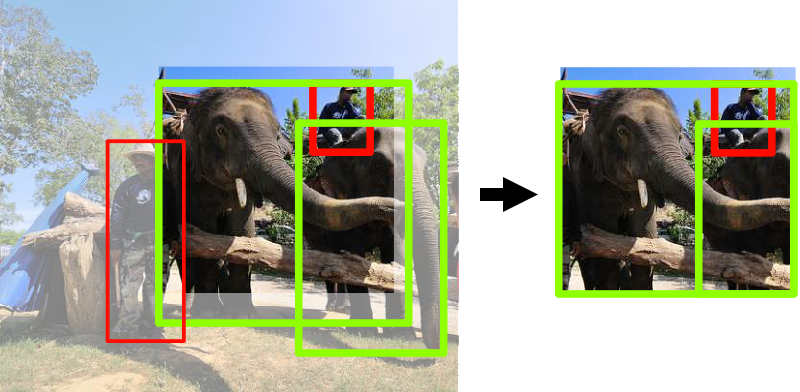
\includegraphics[max width=1\linewidth]{ilustracije/prosirivanje-podataka}
	\caption{Odabir i odbacivanje ciljnih okvira pri uzorkovanju dijela slike. Na lijevoj slici podebljani su svi okviri čije se središta nalaze unutar uzorkovanog područja slike. Oni se zadržavaju i prilagođavaju uzorkovanom dijelu slike.}
	\label{fig:prosirivanje-podataka}
\end{figure}




\chapter{Rezultati} \label{chap:rezultati}

U eksperimentima autori su koristili mrežu VGG-16 s unaprijed naučenim parametrima na skupu podataka \emph{ILSVRC CLS-LOC}. Slojevi \texttt{fc6} i \texttt{fc7} su zamijenjeni konvolucijskim slojevima, \texttt{fc9} uklonjen, a sloj \texttt{pool5} izmijenjen tako da umjesto receptivnog polja dimenzija $2\times2$ i izlaznog koraka $2$ koristi receptivno polje dimenzija $3\times 3$ i izlaznog koraka $1$. 
%TODO a trous

Iskorištavaju se naučeni parametri potpuno povezanih slojeva \texttt{fc6} i \texttt{fc7}. \texttt{fc6} je pretvoren u ekvivalentni konvolucijski sloj s jezgrom\footnote{Ovdje se koristi riječ \emph{jezgra} u jednini, ali ona se zapravo odnosi na $1024$ jezgre jer izvorni sloj \texttt{fc6} ima izlaz dimenzije $1024$.} dimenzija $7\times 7$ koja pokriva cijeli tenzor značajki sloja \texttt{pool5}. Promjenom izlaznog koraka sloja \texttt{pool5} s $2$ na $1$, kako bi imali smisla parametri sloja \texttt{fc6}, potrebno je povećati njegov ulazni korak (dilataciju) na 2, čime se njegovo receptivno polje udvostručuje na dimenzije $14\times 14$ (proporcionalno povećanju dimenzija sloja \texttt{pool5}). Konačno, jezgra sloja \texttt{fc6} je poduzorkovana tako da se pretvori u jezgru dimenzija $3\times 3$ s dilacijom 6, čime se dimenzije receptivnog polje ne mijenjaju. Time se postiže otprilike $20$-postotno ubrzanje prolaza unaprijed u odnosu na mrežu s nepoduzorkovanom jezgrom sloja \texttt{fc6}. Sloj \texttt{fc6} je pretvoren u konvolucijeki sloj s jezgrom domenzija $1\times 1$.

Dodatni slojevi se inicijaliziraju Xavierovim inicijalizacijom. Korišten je stohastički gradijentni spust s koeficijentom inercije (engl. \emph{momentum}) $0.9$, $L^2$ regularizacijom, veličinom grupe $32$, početnom stopom učenja $10^{-3}$ i smanjivanjem stope učenja. Detalji su opisani u radu. Slijedi pregled glavnih rezultata i zaključaka.

Za učenje i testiranje korišteni su skupovi \emph{Pascal VOC2007-test}, \emph{Pascal VOC2012-test} i \emph{COCO}. Usporedba rezultata testiranja različitih modela na prikazana je u tablici~\ref{tab:rezultati-usporedba-map}. Autori zaključuju da SSD ima manju grešku lokalizacije u odnosu na R-CNN jer SSD uči zajednički regresiju i klasifikaciju okvira na istim mapama značajki. R-CNN prvo određuje okvir, uzorkuje dio slike određen okvirom i onda klasificira taj dio slike. 

Autori su također mjerili utjecaj razreda kojemu objekt pripada i veličine objekta. Zaključuju da SSD daje lošije rezultate za male objekte zbog velikog broj slojeva prije prvog sloja čije se mape značajki koriste za lokalizaciju. SSD ima problema kod razlikovanja objekata koji pripadaju nekim razredima (često životinje). Prepoznavanje malih objekata može se poboljšati korištenjem veće ulazne slike, ali autori navode da još ima prostora za poboljšanje. Također zaključuju da SSD zbog razmatranih okvira različitih omjera stranica jako dobro određuje oblik okvira.

% drugačiji rezultati http://host.robots.ox.ac.uk:8080/leaderboard/displaylb.php?cls=mean&challengeid=11&compid=4&submid=9241

\begin{table}[htbp]
	\centering
	\begin{tabular}{|c|c|c|c|c|}
		\hline
		\multirow{2}{*}{Model} & \multirow{2}{*}{\emph{FPS}} & \multirow{2}{*}{Podaci za učenje} & \multicolumn{2}{c|}{$\textit{mAP}/\%$} \\ \cline{4-5}
		& & & VOC2007 & VOC2012 \\
		\hline
		\multirow{2}{*}{Fast-RCNN~\cite{fastrcnn}} 
		& \multirow{2}{*}{0.5}
		& \footnotesize{VOC07} & 66.9 & - \\ \cline{3-5}
		& & \footnotesize{VOC07, VOC12} & 70.0 & 68.4 \\ \hline
		\multirow{3}{*}{Faster-RCNN~\cite{fasterrcnn}}
		& \multirow{3}{*}{7}
		  & \footnotesize{VOC07} & 69.9 & - \\ \cline{3-5}
		& & \footnotesize{VOC07, VOC12} & 73.2 & 70.4 \\ \cline{3-5}
		& & \footnotesize{VOC07, VOC12, COCO} & 78.8 & 75.9 \\ \hline
		YOLO~\cite{yolov2} & 45 & \footnotesize{VOC07, VOC12} & 63.4 & 57.9 \\ \hline
		*YOLOv2-544~\cite{yolov2} & 40 &  \footnotesize{VOC07, VOC12} & 78.6 & 73.4 \\ \hline
		*PVANET-c~\cite{pvanet} & 31 &  \footnotesize{VOC07, VOC12, COCO} & 84.4 & 83.7 \\ \hline
		*PVANET~\cite{pvanet} & 22 &  \footnotesize{VOC07, VOC12, COCO} & 84.9 & 84.2 \\ \hline
		\multirow{3}{*}{SSD300}
		& \multirow{3}{*}{46}
		  & \footnotesize{VOC07} & 68.0 & - \\ \cline{3-5}
		& & \footnotesize{VOC07, VOC12} & 74.3 & 72.1 \\ \cline{3-5}
		& & \footnotesize{VOC07, VOC12, COCO} & 79.6 & 77.5 \\ \hline
		\multirow{3}{*}{SSD512} 
		& \multirow{3}{*}{19} 
		  & \footnotesize{VOC07} & 71.6 & - \\ \cline{3-5}
		& & \footnotesize{VOC07, VOC12} & 76.8 & 74.9 \\ \cline{3-5}
		& & \footnotesize{VOC07, VOC12, COCO} & 81.6 & 80.0 \\ \hline
	\end{tabular}
	\caption{Usporedba rezultata evaluacije na skupovima \emph{VOC2007-test} i \emph{VOC2012-test} označenih u tablici s "VOC2007" i "VOC2012". U stupcu "\emph{FPS}" su brzine izvođenja (broj slika u sekundi) pri pojedinačnoj obradi (grupe veličine $1$) na grafičkoj kartici \emph{Nvidia Titan X}. U stupcu U stupcu "Podaci za učenje" su skupovi podataka (bez dijela koji je korišten za testiranje) koji su korišteni za učenje. "{\footnotesize{VOC07, VOC12, COCO}}" označava da je model (osim za PVANET) prvo učen na skupu \emph{COCO-trainval35k}, a nakon toga još prilagođen na uniji odgovarajućih dijelova skupova \emph{VOC2007} i \emph{VOC2012}. Od različitih varijanti modela, odabrane su one koje su po brzini izvođenja najusporedivije s modelom SSD. * označava modele novije od SSD-a.\cite{ssd,pvanet,yolov2}}
	\label{tab:rezultati-usporedba-map}
\end{table}

Autori su analizirali utjecaj izmjene različitih komponenata na učinak sustava. U tablici~\ref{tab:kanaliza-komponenata} prikazan je utjecaj različitih odabira komponenata na učinak modela SSD300 na skupu\emph{VOC2007-test}. Vidi se da od navedenog, osim korištenja $6$ slojeva značajki u odnosu na samo \texttt{conv7} kao ulaze slojeva za pronalaženje objekata, najveći utjecaj ima dodatno proširivanje skupa podataka u odnosu na korištenje samo originalnih slika i slika dobivenih njihovim horizontalnim zrcaljenjem. Vidi se da značajan utjecaj ima i korištenje okvira s omjerima stranica $\left\{2,3,\frac{1}{2},\frac{1}{3}\right\}$. Korištenje poduzorkovanih jezgri u sloju \texttt{fc6} nema značajan utjecaj na rezultate, ali donosi ubrzanje izvođenja.

\begin{table}
	\centering
	\begin{tabular}{|r|cccccc|}
		\hline
		više slojeva značajki za traženje objekata & & $\bullet$ & $\bullet$ & $\bullet$ & $\bullet$ & $\bullet$ \\
		više proširivanja podataka & $\bullet$ & & $\bullet$ & $\bullet$ & $\bullet$ & $\bullet$ \\
		korištenje omjera $\left\{\frac{1}{2},2\right\}$ & $\bullet$ & $\bullet$ & & $\bullet$ & $\bullet$ & $\bullet$ \\
		korištenje omjera $\left\{\frac{1}{3},3\right\}$ & $\bullet$ & $\bullet$ & & & $\bullet$ & $\bullet$ \\
		jezgra $3\times 3$ s dilatacijom 6 u sloju \texttt{fc6} & $\bullet$ & $\bullet$ & $\bullet$ & $\bullet$ & & $\bullet$ \\
		\hline
		$\textit{mAP}/\%$ & 62.4 & 65.5 & 71.6 & 73.7 & 74.2 & \textbf{74.3} \\
		\hline
	\end{tabular}
	\caption{Utjecaj različitih odabira komponenata na srednju prosječnu pogrešku kod modela SSD300 na skupu \emph{VOC2007-test}. Redak "više slojeva značajki za traženje objekata" označava korištenje slojeva značajki \texttt{conv4\_3}, \texttt{conv7}, \texttt{conv8\_2}, \texttt{conv9\_2}, \texttt{conv10\_2} i \texttt{conv11\_2} umjesto samo \texttt{conv7} za pronalaženje objekata.}
	\label{tab:kanaliza-komponenata}
\end{table}

Na slici~\ref{fig:primjeri-rezultata-detekcije} su prikazani primjeri rezultata pronalaženja objekata modelom SSD500.

\begin{figure}
	\centering
	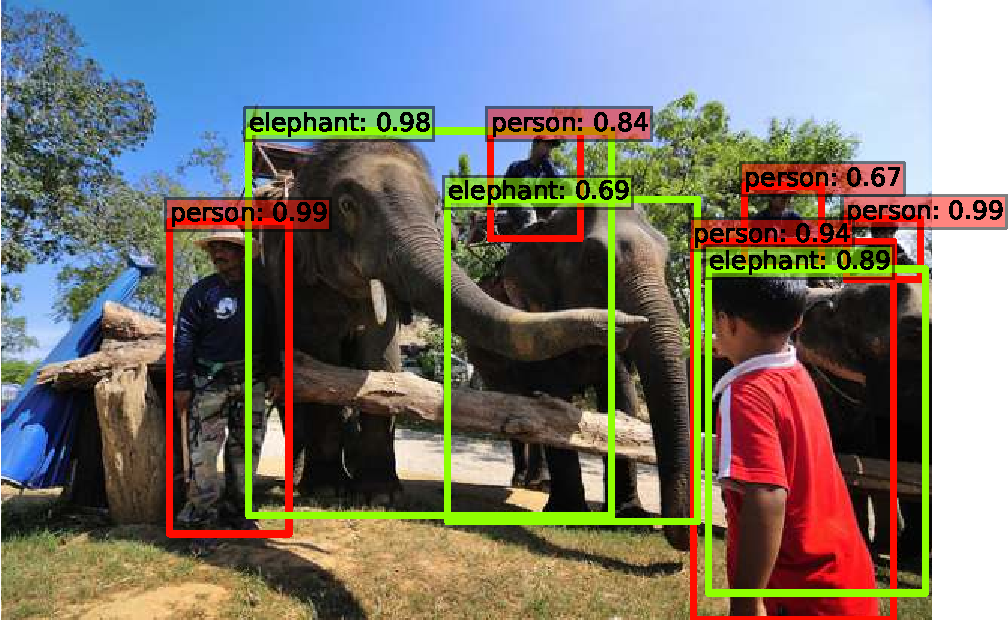
\includegraphics[trim={0 0 0 0.6cm},clip,width=0.24\linewidth]{ilustracije/coco/388513}
	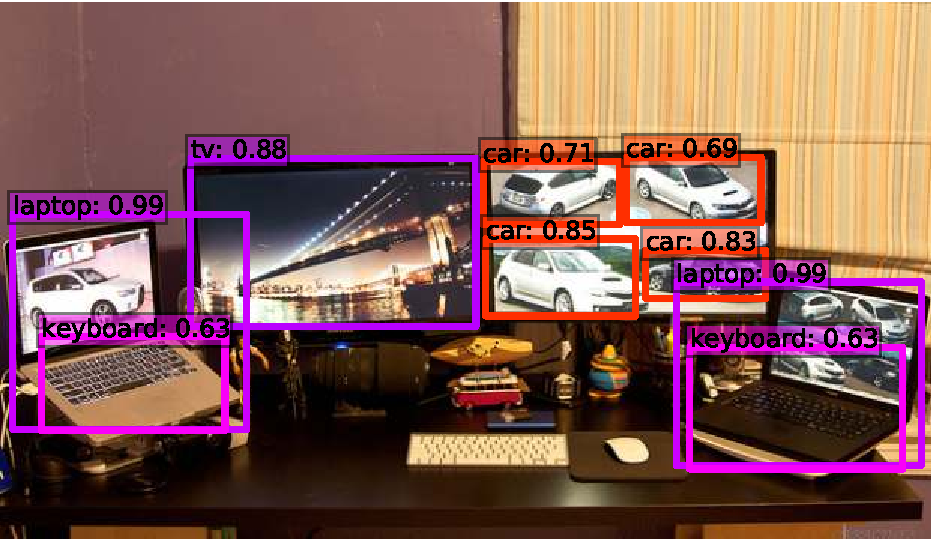
\includegraphics[width=0.24\linewidth]{ilustracije/coco/420454}
	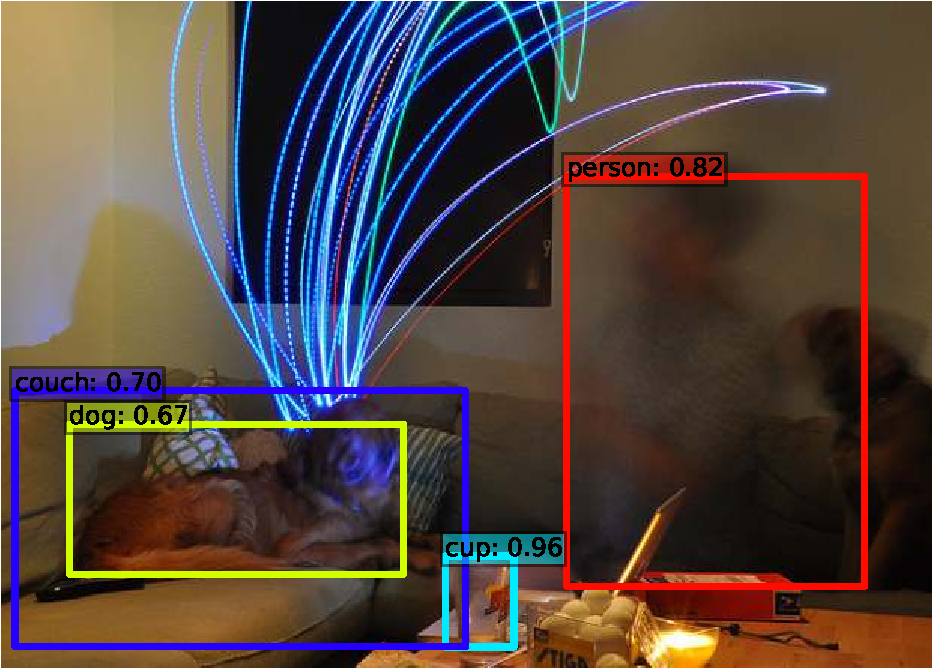
\includegraphics[trim={0 0 0 2.2cm},clip,width=0.24\linewidth]{ilustracije/coco/230476}
	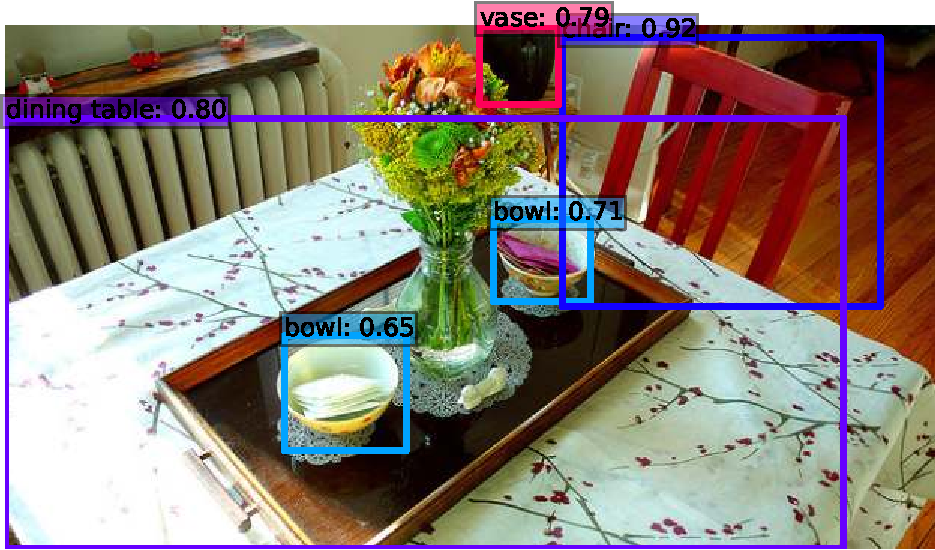
\includegraphics[width=0.24\linewidth]{ilustracije/coco/96709}\\
	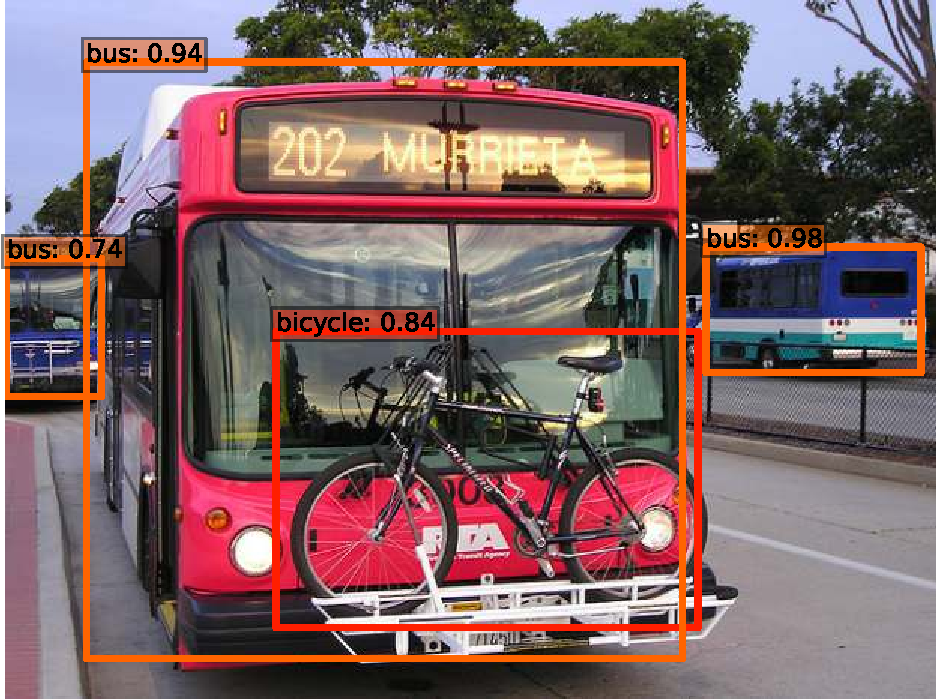
\includegraphics[width=0.24\linewidth]{ilustracije/coco/440980}
	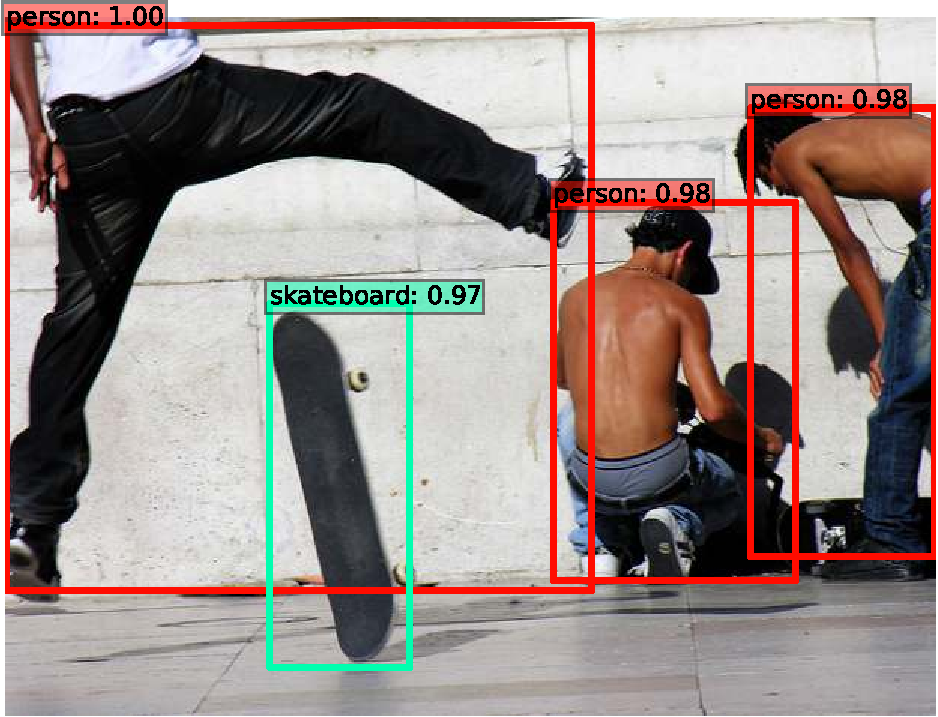
\includegraphics[width=0.24\linewidth]{ilustracije/coco/402750}
	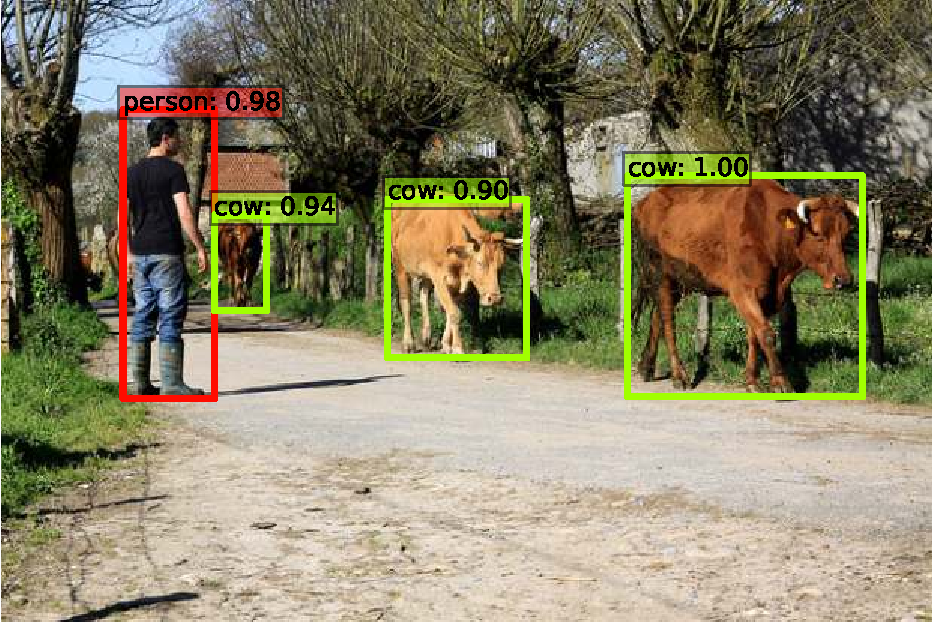
\includegraphics[width=0.24\linewidth]{ilustracije/coco/271809}
	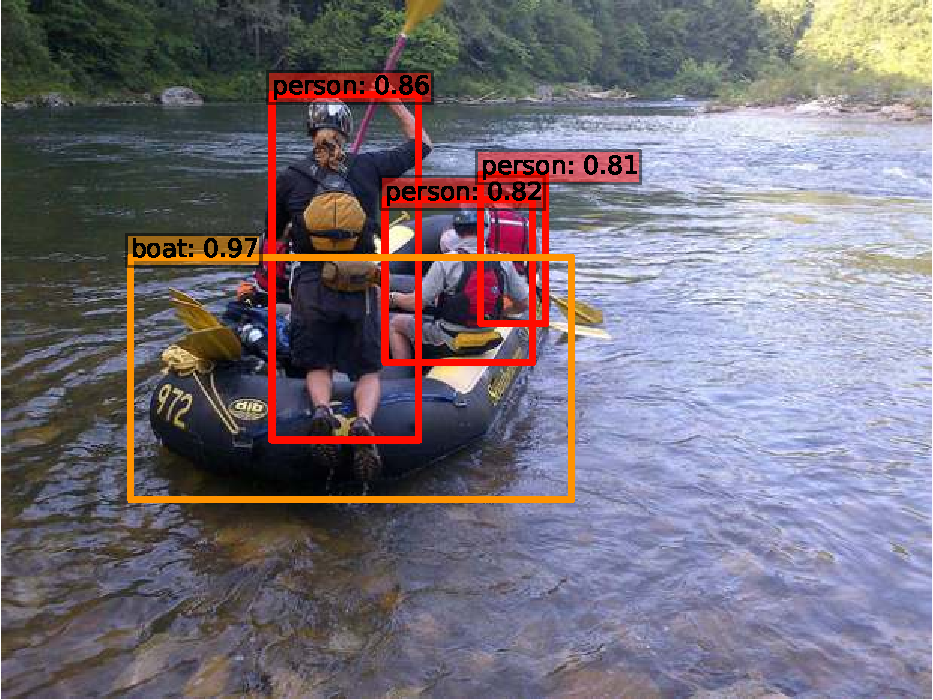
\includegraphics[width=0.24\linewidth]{ilustracije/coco/442079}\\
	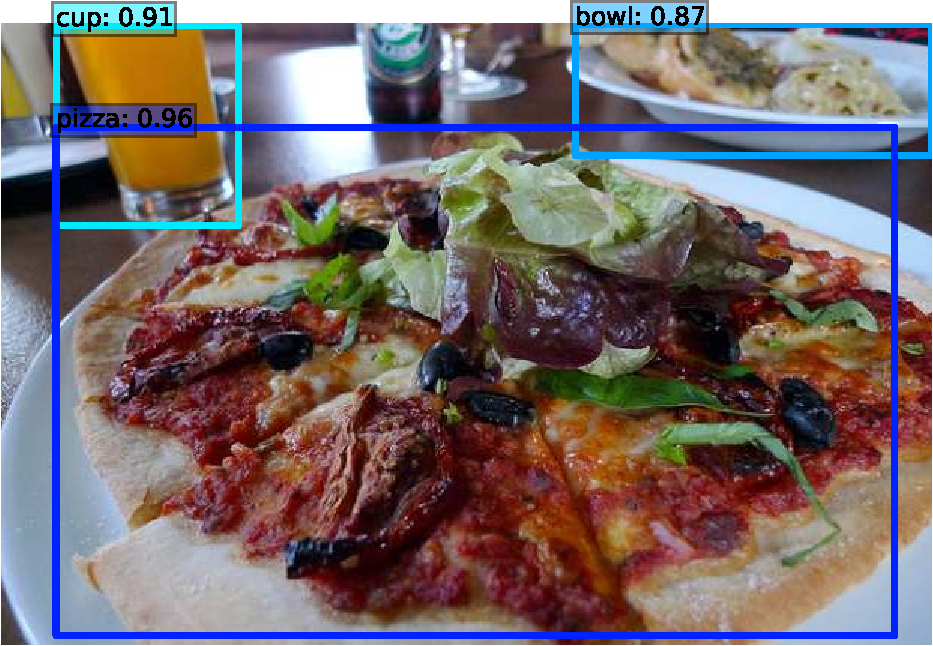
\includegraphics[width=0.24\linewidth]{ilustracije/coco/39662}
	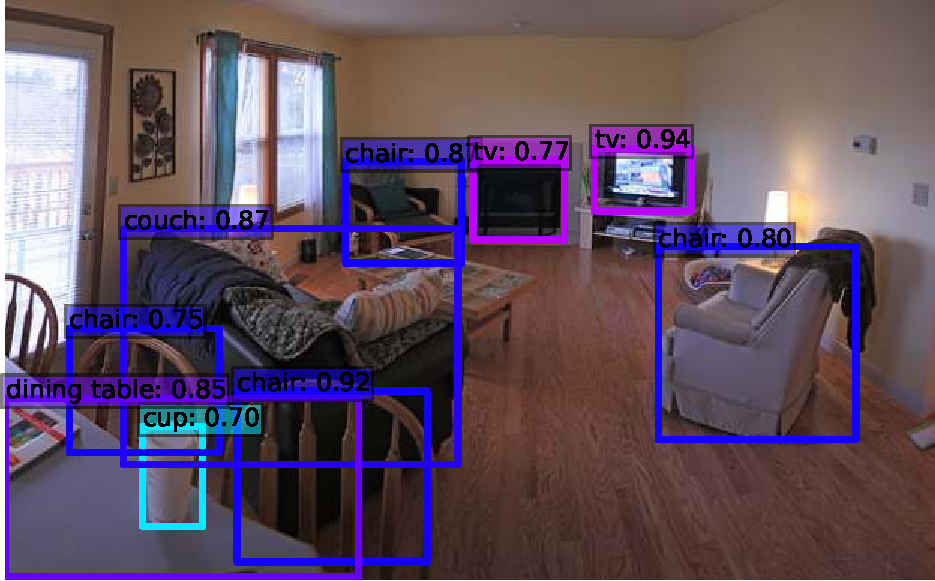
\includegraphics[width=0.24\linewidth]{ilustracije/coco/153988}
	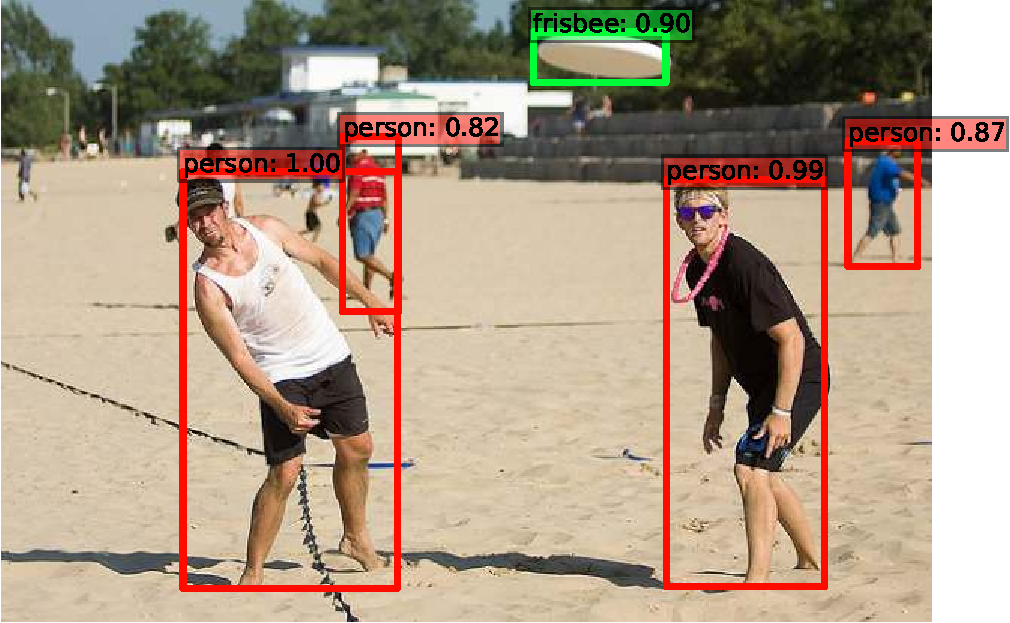
\includegraphics[width=0.24\linewidth]{ilustracije/coco/35114}
	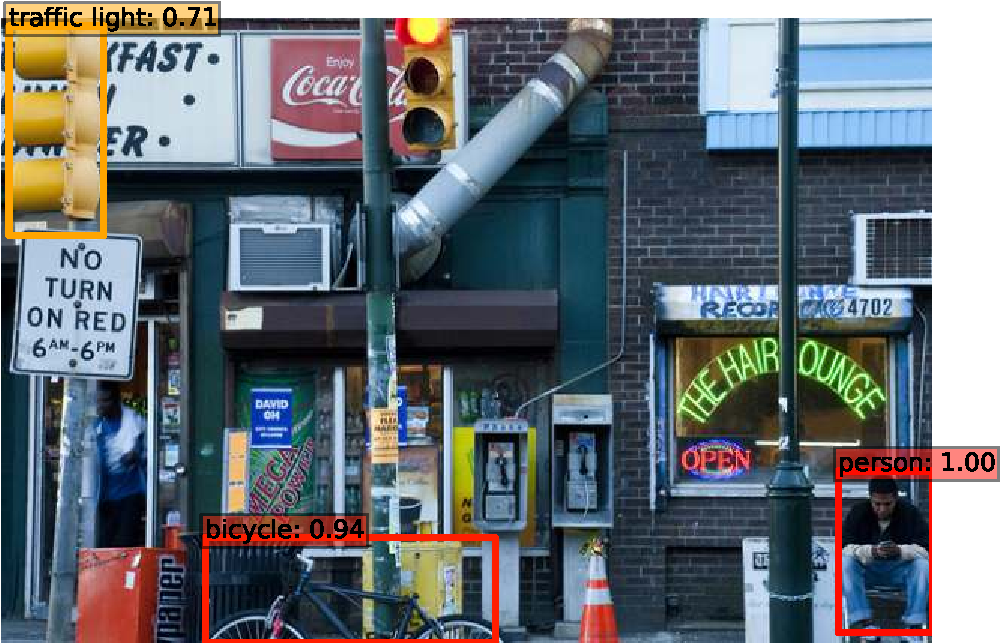
\includegraphics[width=0.24\linewidth]{ilustracije/coco/44974}\\
	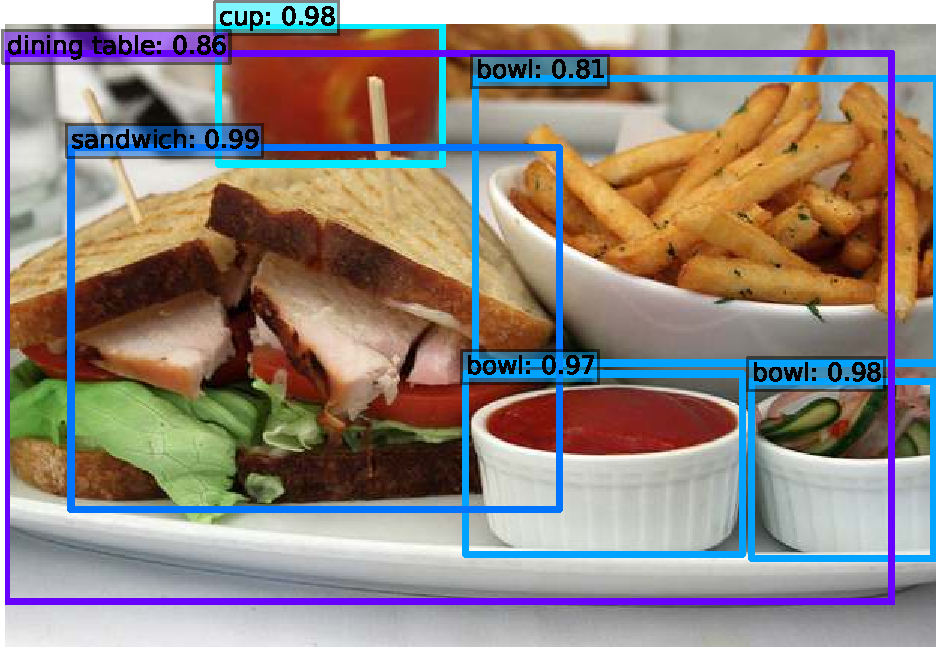
\includegraphics[width=0.24\linewidth]{ilustracije/coco/25090}
	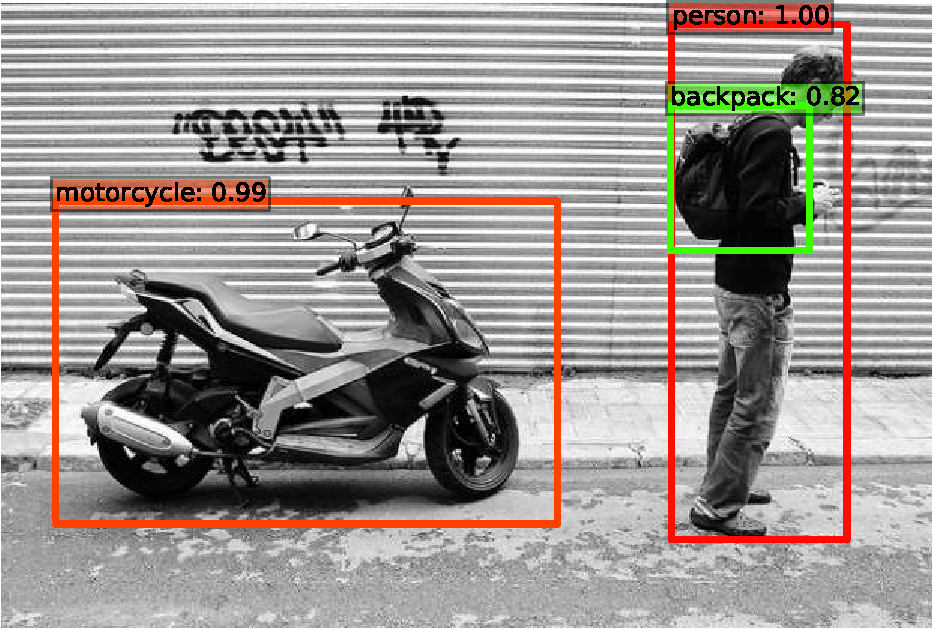
\includegraphics[width=0.24\linewidth]{ilustracije/coco/97838}
	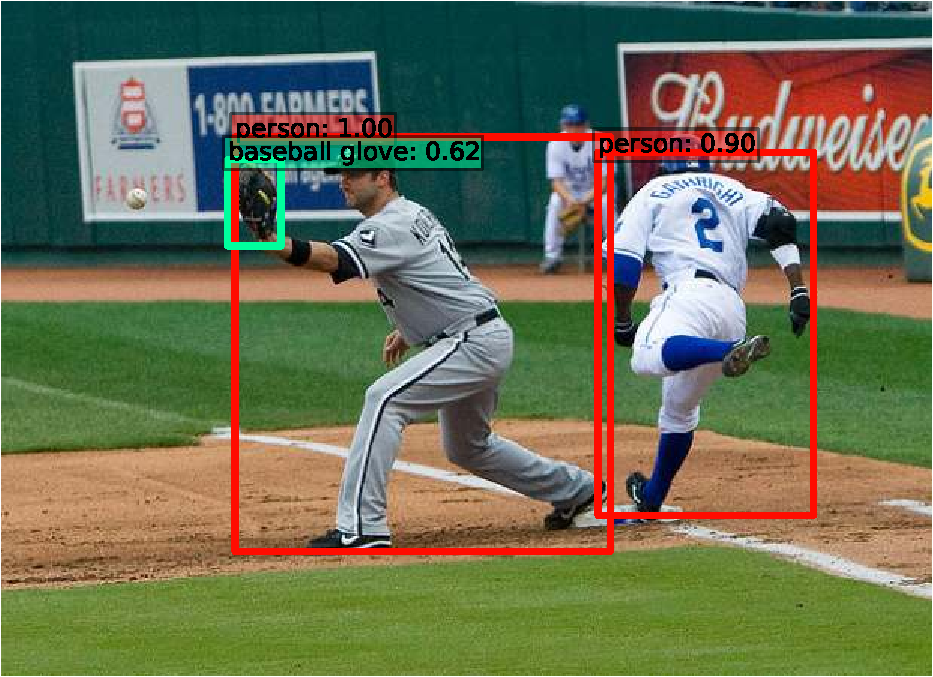
\includegraphics[trim={0 1.0cm 0 0},clip,width=0.24\linewidth]{ilustracije/coco/116280}
	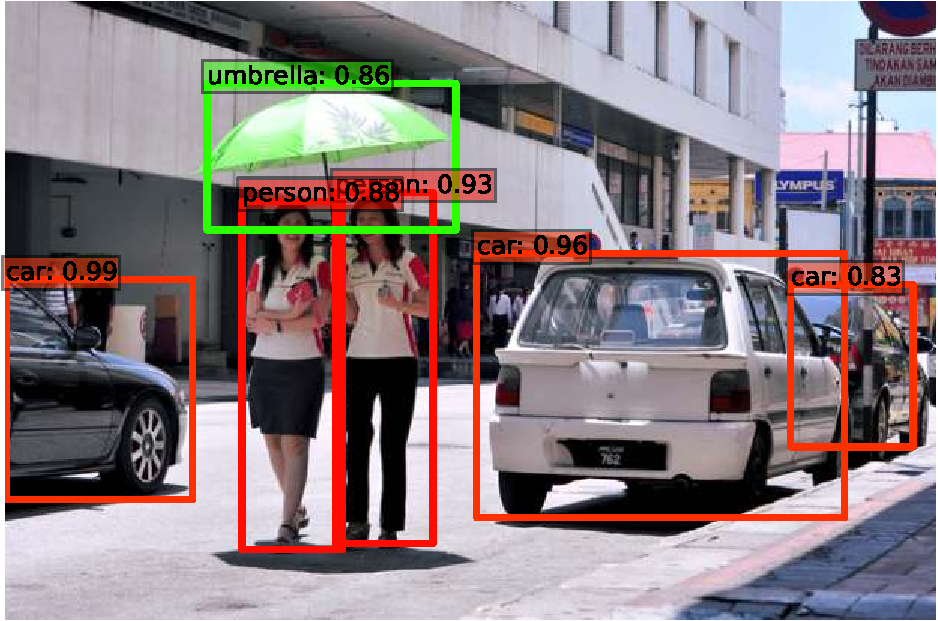
\includegraphics[width=0.24\linewidth]{ilustracije/coco/567767}\\
	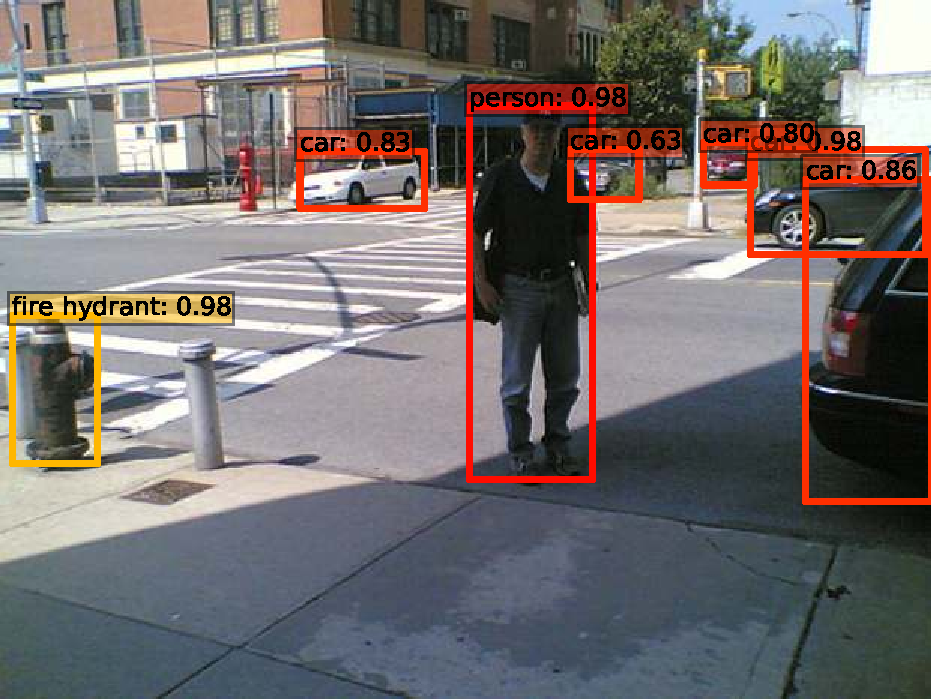
\includegraphics[width=0.24\linewidth]{ilustracije/coco/531694}
	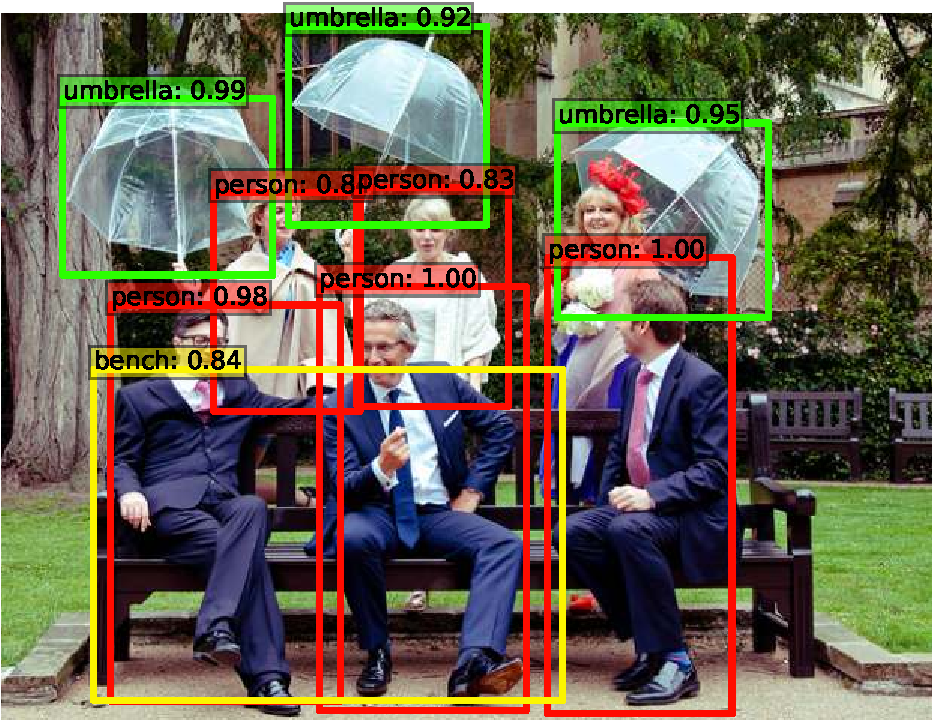
\includegraphics[width=0.24\linewidth]{ilustracije/coco/371251}
	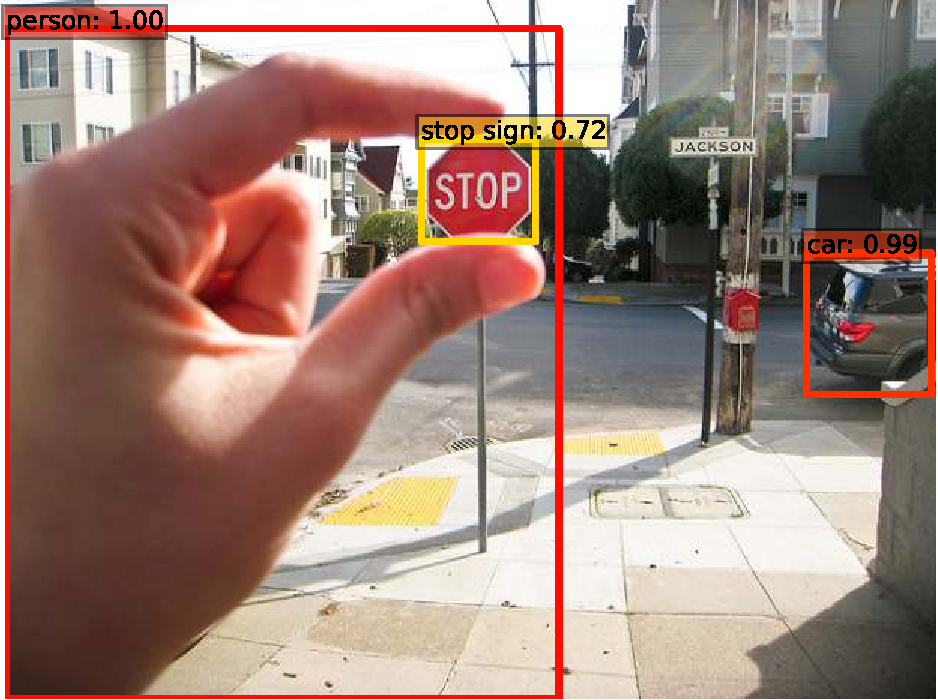
\includegraphics[width=0.24\linewidth]{ilustracije/coco/569617}
	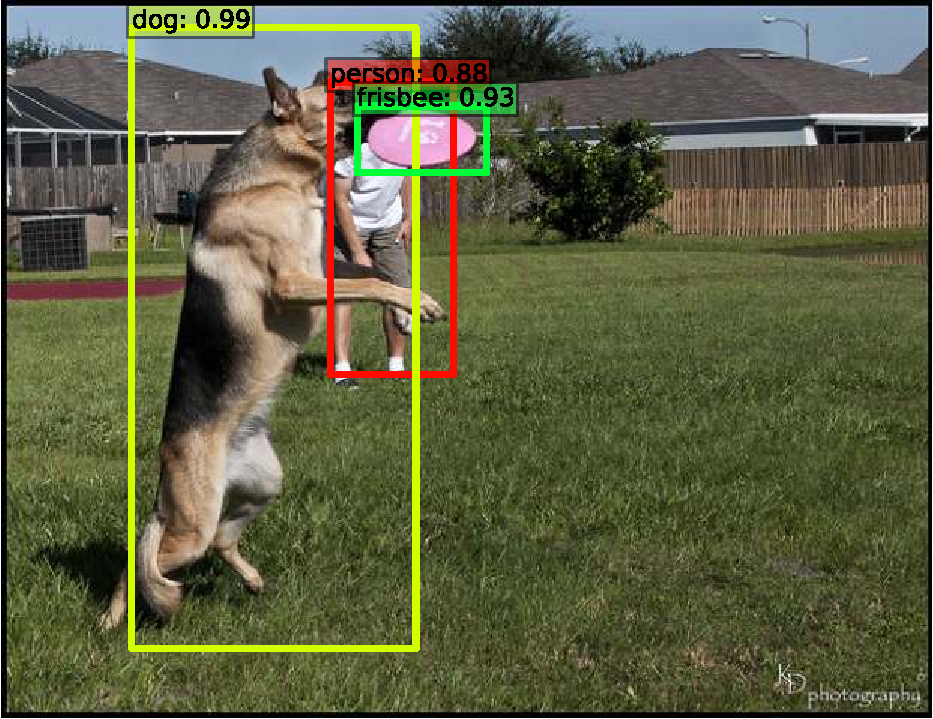
\includegraphics[width=0.24\linewidth]{ilustracije/coco/222239}\\
	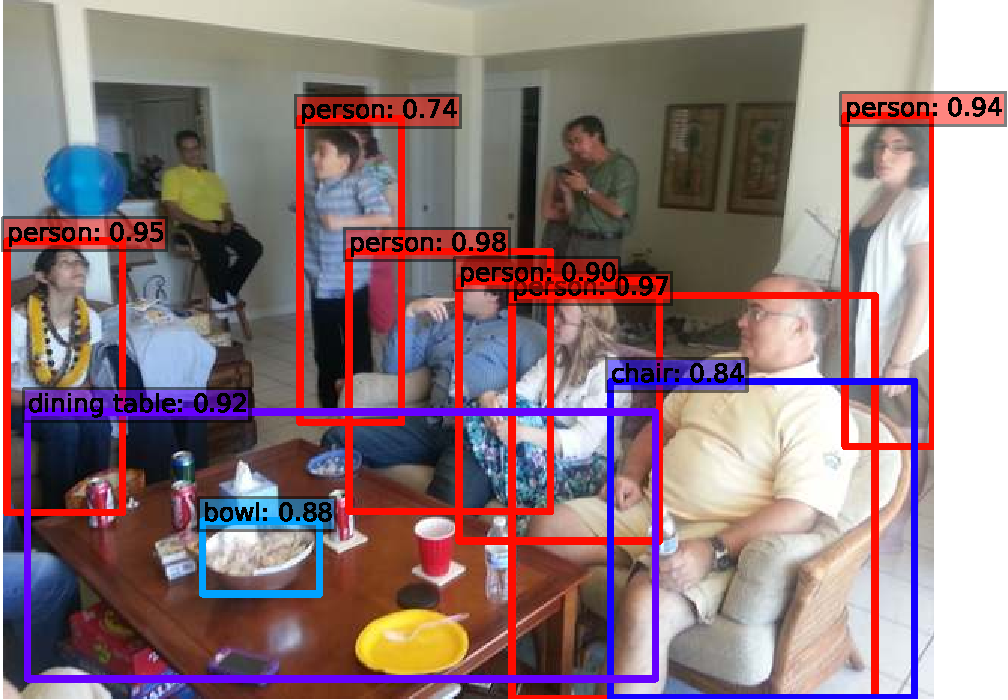
\includegraphics[trim={0 0 0 0.4cm},clip,width=0.24\linewidth]{ilustracije/coco/474449}
	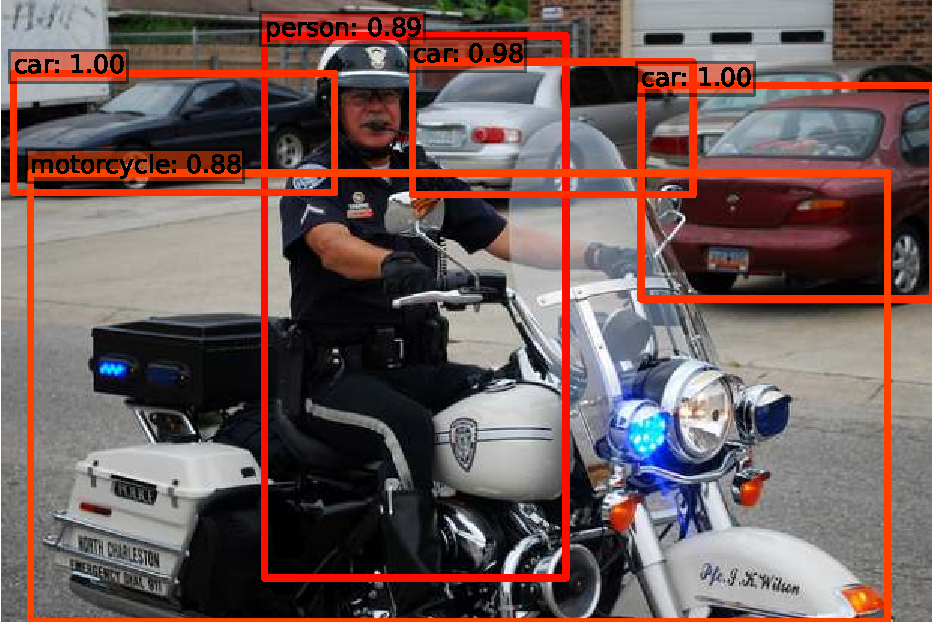
\includegraphics[width=0.24\linewidth]{ilustracije/coco/145416}
	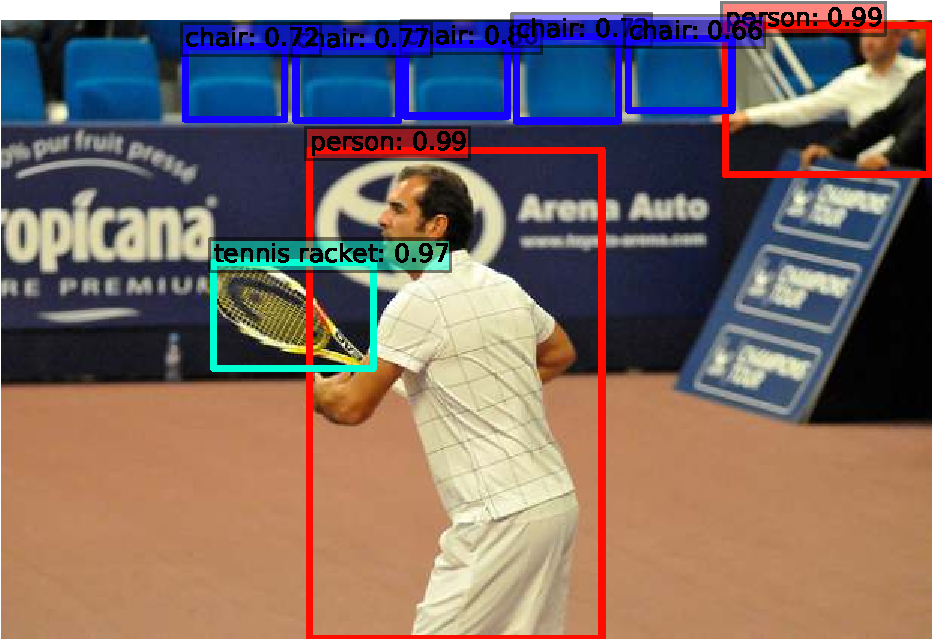
\includegraphics[width=0.24\linewidth]{ilustracije/coco/237488}
	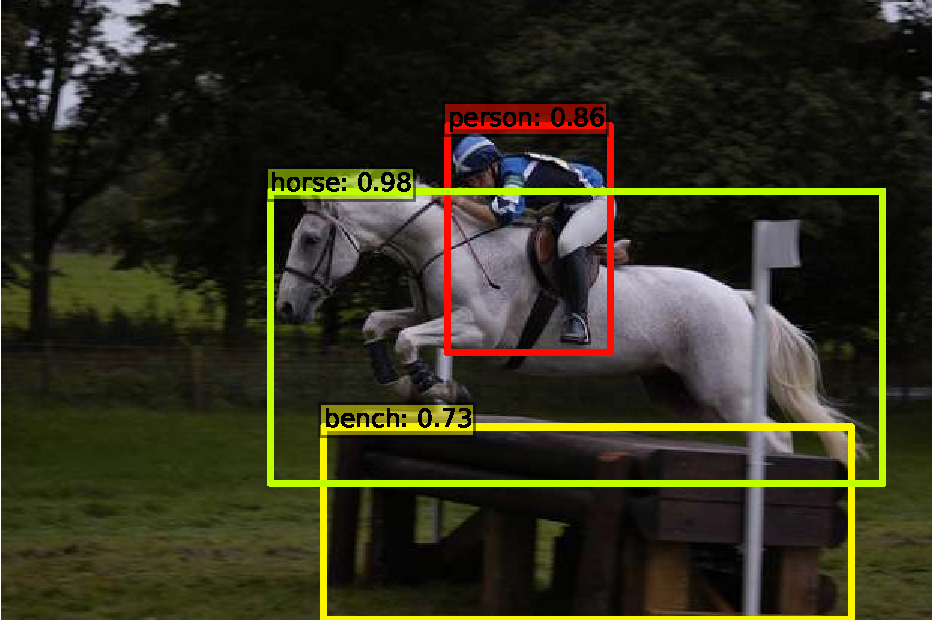
\includegraphics[width=0.24\linewidth]{ilustracije/coco/147107}\\
	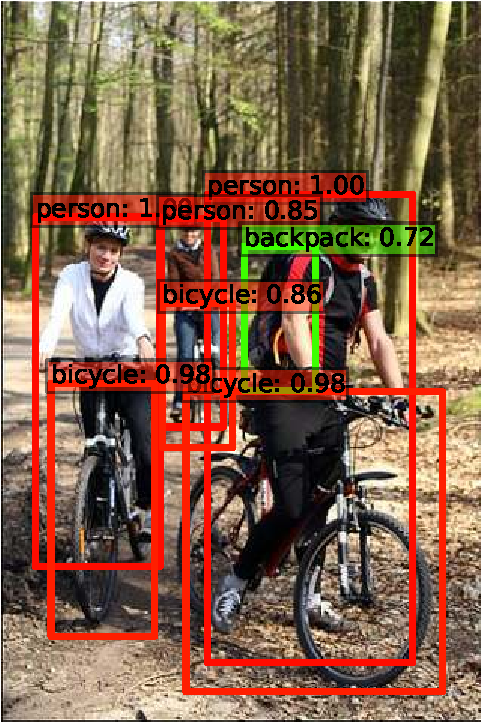
\includegraphics[width=0.24\linewidth]{ilustracije/coco/461193}
	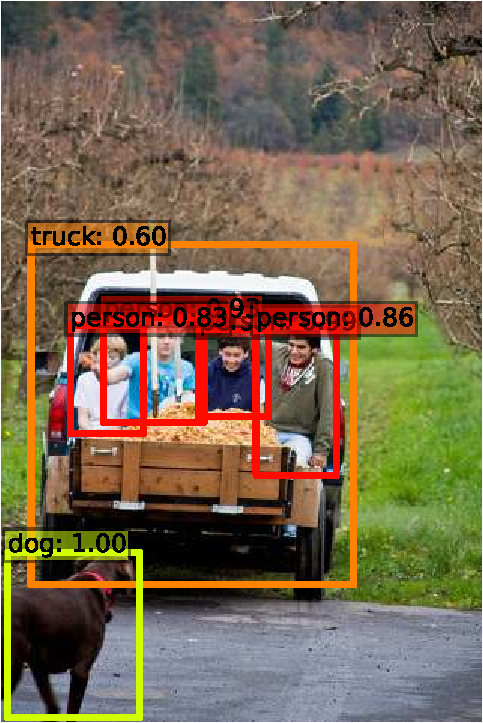
\includegraphics[width=0.24\linewidth]{ilustracije/coco/23408}
	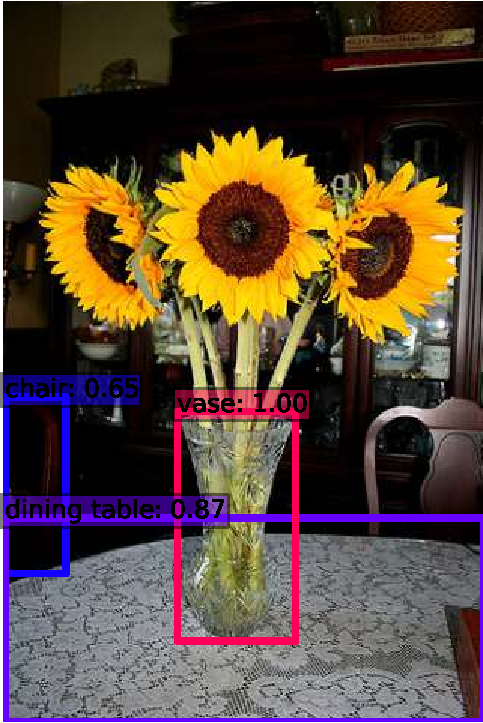
\includegraphics[width=0.24\linewidth]{ilustracije/coco/33705}
	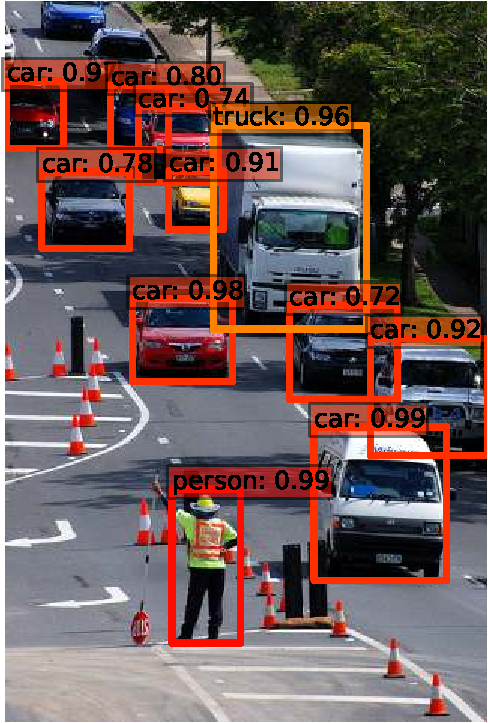
\includegraphics[width=0.24\linewidth]{ilustracije/coco/61871}\\
	\caption{Primjeri rezultata pronalaženja objekata na slikama iz skupa \emph{COCO-test-dev} modelom SSD500. Prikazani su okviri s pouzdanošću klasifikacije većom od $0.6$. Slike su preuzete iz \cite{ssd}.}
	\label{fig:primjeri-rezultata-detekcije}
\end{figure}


\chapter{Zaključak} \label{chap:zakljucak}

SSD donosi neke zanimljive ideje koje zajedno omogućuju brzu obradu slika bez smanjenja kvalitete rezultata u odnosu na neke druge modele. Glavne od njih su korištenje slojeva značajki različitih dimenzija na različitima dubinama konvolucijske mreže za pronalaženje objekata i korištenje razmatranih okvira različitih omjera stranica kao osnova za dobivanje konačnih okvira združenom regresijom i klasifikacijom. Time je postignuta relativno jednostavna konvolucijska arhitektura kojom se izbjegavaju višestruki izračuni sličnih značajki i omogućuje dobro prepoznavanje objekata različitih veličina i oblika. 

U prepoznavanju objekata, kao i mnogim drugim područjima računalnog vida, još uvijek nisu postignuti rezultati koji dostižu one koje postižu ljudi. Ima puno prostora za poboljšanje i može se očekivati još poboljšanja nad postojećim modelima.

\begin{sazetak}
	Ovaj seminar razmatra postupak pronalaženja orijentiranih okvira (engl. oriented bounding box, OBB) koji obuhvaćaju objekte koji pripadaju različitim kategorijama na slici. Postupak \emph{Single Shot MultiBox Detector} (SSD) objavljen je $2016$. i donosi višestruko ubrzanje učenja i izvođenja bez gubitka preciznosti (mAP) s obzirom na dotadašnje najbolje modele Fast R-CNN i Faster R-CNN. 
	
	\kljucnerijeci{lokalizacija objekata, računalni vid, konvolucijske mreže, duboke neuronske mreže, duboko učenje}
\end{sazetak}

%\engtitle{SSD Object Localization}
%\begin{abstract}
%\end{abstract}


\bibliography{literatura}
\bibliographystyle{fer}

\nocite{colah}
\nocite{nndl}


\end{document}
